\section{System Design}
\label{sec:sys-design}

Building on the requirements and behavioural models identified in Section~\ref{sec:sys-analysis}, this section presents the proposed design of BK Uni and explains how each design decision addresses the needs of its stakeholders. It covers the system architecture, the database design and the user-interface design. Together, they form a clear specification for implementing a system that is correct with respect to curriculum rules, maintainable as curricula change, and able to explain its results to Students.

\subsection{Architecture Designs}
\label{subsec:architecture-design}

A platform such as BK Uni brings together several kinds of work that behave very differently: ordinary data management (profiles, curricula, course statuses), rule-based reasoning over a whole curriculum to analyze progress and recommend study plans, and conversational advising backed by a large language model. A well-defined architecture is needed to organize these concerns into one cohesive system. Without it, the dependencies between the curriculum data, the planning solvers that interpret academic rules, and the external AI service would quickly become difficult to reason about, test and evolve, which would directly threaten the correctness and explainability that the system promises.

This section presents the architecture of the platform: what software architecture means, the common architectural styles that were considered, the architectural decision made for BK Uni, and the resulting architecture design.

\subsubsection{Software Architectures}
\label{subsubsec:software-architecture}

Software architecture is the high-level structural design of a software system. It determines how the system is decomposed into components, how those components interact, how data flows between them, and how the system can grow over time. At its core, architecture is about the significant decisions that are difficult and costly to change later. For BK Uni, this means deciding, before any feature is implemented, where academic rules are evaluated, how curriculum and student data reach the planning solvers, and how the AI advisor is allowed to access that data.

Several authoritative definitions of software architecture are commonly cited:
\begin{itemize}
    \item \textbf{ISO/IEC/IEEE 42010:2011} (formerly IEEE 1471) defines architecture as the ``fundamental concepts or properties of a system in its environment embodied in its elements, relationships, and in the principles of its design and evolution''~\cite{iso42010}.
    \item \textbf{The Software Engineering Institute (SEI) at Carnegie Mellon University} describes it as the ``set of structures needed to reason about the system, which comprise software elements, relations among them, and properties of both''~\cite{bass-sei}.
    \item \textbf{The Open Group Architecture Framework (TOGAF)} gives two interpretations: (1) ``a formal description of a system, or a detailed plan of the system at component level to guide its implementation'', and (2) ``the structure of components, their inter-relationships, and the principles and guidelines governing their design and evolution over time''~\cite{togaf}.
    \item \textbf{Ralph Johnson}, one of the ``Gang of Four'', offers a pragmatic industry view, describing architecture as ``the decisions that you wish you could get right early in a project''~\cite{fowler-architect}.
\end{itemize}

Based on these definitions, software architecture can be characterized by three essential pillars:
\begin{itemize}
    \item \textbf{Structure:} the logical and physical components of the system and how they are organized and partitioned to manage complexity.
    \item \textbf{Behaviour:} the interaction patterns between components, including the protocols and data exchanged between them.
    \item \textbf{Quality attributes:} beyond functionality, the architecture must address non-functional requirements such as security, performance, reliability, maintainability and scalability (Section~\ref{sec:sys-analysis}).
\end{itemize}

\subsubsection{Common Architectural Styles}
\label{subsubsec:architecture-styles}

Selecting an architectural style is a critical decision because it determines how the platform handles data, isolates complex logic and scales over time. Architectural styles are generally divided into \emph{monolithic} styles, in which all components are deployed as a single unit, and \emph{distributed} styles, in which components are deployed separately and communicate over a network~\cite{richards-ford}.

\textbf{Monolithic architecture styles}
\begin{itemize}
    \item \textbf{Layered architecture (n-tier):}
    \begin{itemize}
        \item \textit{Definition:} organizes the application into horizontal layers (for example presentation, business, persistence and database), each with a specific role and interacting only with the layer directly below it.
        \item \textit{Best for:} small to medium applications where development speed matters and the domain is not overly complex.
    \end{itemize}
    \item \textbf{Pipeline architecture (pipe-and-filter):}
    \begin{itemize}
        \item \textit{Definition:} decomposes a task into a sequence of self-contained processing steps (filters) connected by channels (pipes).
        \item \textit{Best for:} systems dominated by data transformation, such as document processing, ETL jobs or compilers.
    \end{itemize}
    \item \textbf{Microkernel architecture (plug-in):}
    \begin{itemize}
        \item \textit{Definition:} consists of a minimal core system and a set of plug-in modules that provide specialized features or additional logic.
        \item \textit{Best for:} products in which custom extensions must be added without modifying the core.
    \end{itemize}
\end{itemize}

\textbf{Distributed architecture styles}
\begin{itemize}
    \item \textbf{Service-based architecture:}
    \begin{itemize}
        \item \textit{Definition:} a hybrid approach in which the application is split into a small number of coarse-grained, independently deployed services that typically share a single database.
        \item \textit{Best for:} systems that need to isolate a few distinct domains or runtimes without taking on the full operational complexity of a fine-grained distributed system.
    \end{itemize}
    \item \textbf{Event-driven architecture:}
    \begin{itemize}
        \item \textit{Definition:} an asynchronous style in which components communicate by producing and consuming events through a broker, yielding highly decoupled and reactive systems.
        \item \textit{Best for:} high-throughput systems with real-time updates or long-running asynchronous workflows.
    \end{itemize}
    \item \textbf{Microservices architecture:}
    \begin{itemize}
        \item \textit{Definition:} many small, fine-grained services, each owning its own database and communicating through lightweight protocols such as HTTP or gRPC.
        \item \textit{Best for:} large, complex systems that require independent scaling and deployment of many features and high fault tolerance.
    \end{itemize}
\end{itemize}

\subsubsection{Strategic Decision}
\label{subsubsec:architecture-decision}

Among the styles listed above, BK Uni adopts a \textbf{modular, layered monolith} for its server, extended with \textbf{out-of-process Python workers} for the CPU-bound work. The \emph{Backend Server} is a single deployable application that owns all business data and exposes every function of the system. When a request needs combinatorial search or document parsing, the Backend starts a short-lived Python process, the \emph{planner}, passes it the input as JSON on its standard input, and reads the result from its standard output. This keeps the operational simplicity of a monolith while isolating the parts that differ most from ordinary request handling, and it follows directly from the nature of the problem:
\begin{itemize}
    \item \textbf{Different runtimes and workloads.} The Backend Server performs short, I/O-bound operations (database reads and writes, calls to the AI service), for which Node.js is well suited. Building a study roadmap is a CPU-bound search over a whole curriculum, and the mature solvers for it, Google OR-Tools CP-SAT and \texttt{clingo}, are available in Python. Running each solving step in its own process keeps it from blocking the request-handling event loop, lets each part use the most suitable language, and allows the Backend to stop a solver that runs too long.
    \item \textbf{Separation of rules from application code.} The planning problem is defined once as a constraint satisfaction problem (Section~\ref{sec:formulation}) and implemented in the planner, not in the Backend. The planner has two interchangeable solver back-ends: a CP-SAT model, used by the Student interface, and an Answer Set Programming encoding (Section~\ref{sec:encoding}) solved by \texttt{clingo}, available through the same API for comparison. Rules can therefore be developed and tested in Python on fixed inputs without touching the rest of the application, which supports NFR-4.1 and NFR-4.2.
    \item \textbf{Stateless workers with a single data owner.} A planner process never accesses the database. It receives everything it needs for one request and exits after replying, so the Backend Server remains the only component that reads and writes persistent data and enforces authentication and data ownership on every request (NFR-1.1). This avoids the data-consistency and infrastructure overhead of a database per service, which matters for a small development team.
\end{itemize}

Within the Backend Server, the code follows a modular, layered design: each functional area (authentication, users, student data, curricula, courses, course outlines, planning and the AI advisor) is a self-contained module with its own controllers, services and data entities. This keeps responsibilities clear while avoiding the cost of splitting every module into its own service. Two kinds of work are deliberately kept out of the server. The \emph{progress analysis} of a Student is computed in the browser from data the Backend serves, because it must react instantly to unsaved edits on the course board. \emph{Data ingestion} follows the pipeline style: curricula and course outlines are fetched from the university's systems and transformed offline before being imported into the system.

An event-driven design with a message broker was deliberately not adopted at this stage. Planning requests are bounded in size, since a single curriculum contains a few hundred courses: the CP-SAT search is limited to 20 seconds and any planner process is stopped after 60 seconds. A synchronous request--response interaction is therefore simpler, easier to debug and sufficient. Because the Backend talks to the planner through a narrow JSON interface, the workers could later be moved behind a queue or onto separate machines without changing the Backend's business modules, should the load require it.

\subsubsection{Architecture Design}
\label{subsubsec:architecture-overview}

The design follows a client--server model in which a single-page frontend communicates with the Backend Server, and the Backend Server in turn delegates roadmap planning and report parsing to Python workers and conversational advising to an external language model. The design pursues three main goals: keeping the academic rules of planning in one place that can be tested independently; ensuring that persistent data is accessed and protected by exactly one component; and integrating the external AI service in a controlled way so that it can only use data the system provides.

Figure~\ref{fig:system-architecture} shows the overall architecture of BK Uni.

\begin{figure}[H]
    \centering
    % Fixed font sizes so the diagram does not depend on the 14pt body font
    \renewcommand{\small}{\fontsize{9}{11}\selectfont}%
    \renewcommand{\scriptsize}{\fontsize{7}{8.5}\selectfont}%
    \resizebox{\textwidth}{!}{%
    \begin{tikzpicture}[
        font=\small,
        >=stealth,
        comp/.style={draw, thick, align=center, fill=white, inner sep=3pt},
        ext/.style={comp, fill=gray!8},
        store/.style={draw, thick, cylinder, shape border rotate=90, aspect=0.22,
                      align=center, minimum width=3.2cm, minimum height=1.9cm, fill=white},
        flow/.style={->, thick},
        lbl/.style={font=\scriptsize, fill=white, inner sep=1.5pt, align=center},
      ]
      % ---------------- Containers ----------------
      \draw[thick] (2.6,10.1) rectangle (12.6,11.9);
      \draw[thick] (3.1,10.1) -- (3.1,11.9);
      \node[rotate=90, font=\bfseries\small] at (2.85,11.0) {Clients};
      \draw[thick] (2.6,5.4) rectangle (12.6,8.1);
      \draw[thick] (3.1,5.4) -- (3.1,8.1);
      \node[rotate=90, font=\bfseries\small] at (2.85,6.75) {Servers};
      \draw[thick] (13.4,7.9) rectangle (18.6,11.1);
      \draw[thick] (13.4,10.5) -- (18.6,10.5);
      \node[font=\bfseries\small] at (16.0,10.8) {External Services};

      % ---------------- Components ----------------
      \node[comp, minimum width=9.2cm, minimum height=1.3cm] (fe) at (7.85,11.0)
           {Frontend\\[-1pt]{\scriptsize (React single-page application for Students and Admins;}\\[-2pt]
            {\scriptsize progress analysis computed in the browser)}};

      \node[comp, minimum width=3.9cm, minimum height=2.2cm] (be) at (5.2,6.75)
           {Backend Server\\[-1pt]{\scriptsize (NestJS)}\\[1pt]
            {\scriptsize Auth $\cdot$ User $\cdot$ Student $\cdot$ Curriculum}\\[-2pt]
            {\scriptsize Course $\cdot$ Outline $\cdot$ Planner $\cdot$ Advisor}};

      \node[comp, minimum width=3.7cm, minimum height=2.2cm] (re) at (10.6,6.75)
           {Python Workers\\[-1pt]{\scriptsize (one process per request)}\\[1pt]
            {\scriptsize planner.cli: CP-SAT or clingo}\\[-2pt]
            {\scriptsize planner.mybk: progress reports}};

      \node[comp, minimum width=4.4cm, minimum height=1.8cm] (ds) at (16.0,9.3)
           {DeepSeek API\\[-1pt]{\scriptsize (large language model behind}\\[-2pt]{\scriptsize the AI academic advisor)}};

      \node[ext, minimum width=4.2cm, minimum height=1.8cm] (src) at (-0.5,11.0)
           {myBK\\[-1pt]{\scriptsize (university system: curriculum}\\[-2pt]{\scriptsize API, course outlines)}};

      \node[comp, minimum width=4.2cm, minimum height=2.7cm] (pl) at (-0.5,6.75)
           {Data Ingestion Scripts\\[-1pt]{\scriptsize (offline, Node.js)}\\[1pt]
            {\scriptsize fetch $\cdot$ normalize}\\[-2pt]
            {\scriptsize build import JSON}};

      \node[store] (db) at (4.8,2.3) {PostgreSQL\\Database};
      \node[store, minimum width=3.0cm] (es) at (7.9,2.3) {Search Index\\{\scriptsize (Elasticsearch,}\\[-2pt]{\scriptsize optional)}};
      \node[store] (asp) at (11.4,2.3) {Planning Rules\\{\scriptsize (CP-SAT model,}\\[-2pt]{\scriptsize ASP \texttt{.lp} files)}};

      % ---------------- Flows ----------------
      \draw[flow] (4.6,10.35) -- (4.6,7.85) node[lbl, pos=0.45] {RESTful APIs\\(HTTPS, session cookie)};
      \draw[flow] (7.15,7.15) -- (8.75,7.15) node[lbl, midway, above=1pt, fill=none] {JSON (stdin)};
      \draw[flow] (8.75,6.35) -- (7.15,6.35) node[lbl, midway, below=1pt, fill=none] {JSON (stdout)};
      \draw[flow] (6.4,7.85) |- (ds.west) node[lbl, pos=0.75] {RESTful APIs (tool calling)};
      \draw[flow] (4.8,5.65) -- (db.north) node[lbl, midway] {SQL queries\\(TypeORM)};
      \draw[flow] (7.0,5.65) -- (7.0,3.25) node[lbl, midway] {Outline\\search};
      \draw[flow] (asp.north) -- (11.4,5.65) node[lbl, midway] {Loaded by\\the solvers};
      \draw[flow] (src.south) -- (pl.north) node[lbl, midway] {Fetches JSON\\and outlines};
      \draw[flow] (pl.south) |- (3.5,4.4) -- (3.5,5.65);
      \node[lbl] at (1.5,4.4) {Admin import (RESTful APIs)};
    \end{tikzpicture}%
    }
    \caption{System architecture}
    \label{fig:system-architecture}
\end{figure}

\begin{itemize}
    \item \textbf{Clients (Frontend):} A single-page application built with React that serves as the only user interface for both Students and Admins. It communicates exclusively with the Backend Server through RESTful APIs over HTTPS; it never contacts the database, the Python workers or the AI service directly. Authentication relies on a session token stored in an HTTP-only cookie, so the token is never exposed to client-side scripts (NFR-1.3). Besides rendering, the frontend computes the Student's progress analysis (credit progress, course eligibility, outstanding requirements and personal-plan warnings) from the data the Backend serves, and keeps edits on the course board as a draft until the Student saves them. The interface adapts to the user's role, showing the course board, analysis, roadmap recommendations and the AI advisor to Students, and curriculum management screens to Admins.

    \item \textbf{Servers:} The processing layer consists of the Backend Server and the Python workers it starts:
    \begin{itemize}
        \item \textbf{Backend Server:} The central orchestrator, implemented with NestJS. It handles every client request, authenticates the user, checks role and data ownership, and validates input before any business logic runs; a rate limiter is configured for sign-in and AI requests and must be enabled in production. It is organized into modules: \emph{Auth} (registration, sign-in and server-side sessions), \emph{User}, \emph{Student} (profiles, course statuses, personal plans and regulation statuses), \emph{Curriculum} and \emph{Course} (curricula, elective groups, specializations, categories, course relations and offering history), \emph{Outline} (import and lookup of course outlines), \emph{Planner} (myBK progress import, saved planning scenarios and roadmap solving) and \emph{Advisor} (AI conversations). For a roadmap request, the Planner module loads the Student's record and the curriculum data, builds the solver input, and runs the planner process; for a myBK report, it passes the uploaded bytes to the report reader and stores the parsed progress in a transaction.
        \item \textbf{Python Workers:} Short-lived processes of the \texttt{planner} package, started by the Backend for each request and fed through standard input and output. \texttt{planner.cli} implements the formulation in Section~\ref{sec:formulation}: it normalizes the input, solves it with the CP-SAT model (or with the \texttt{clingo} ASP encoding when that engine is selected), validates the resulting roadmap against the curriculum rules, compares it with the Student's baseline roadmap, and returns the roadmap together with the reason for each course, the assumptions and the warnings. If no roadmap satisfies the constraints, it reports which of the Student's settings block it and proposes fixes instead of relaxing any rule (FR-5.6). \texttt{planner.mybk} reads a myBK progress report, either a PDF or pasted text, into structured JSON. The workers hold no state and no database credentials, so they can be tested in isolation on fixed inputs; the Backend stops any worker that has not replied within 60 seconds.
    \end{itemize}

    \item \textbf{Data and Rule Tier:}
    \begin{itemize}
        \item \textbf{Database:} A PostgreSQL database, with all tables grouped under a dedicated schema, which serves as the system of record for user accounts and sessions, student profiles and academic records, imported myBK progress, curricula, course outlines and import batches, and AI advisor conversations (Section~\ref{subsec:database-design}). Only the Backend Server connects to it, multi-step changes are executed in transactions so that data is never left partially updated (NFR-3.2), and database triggers record changes to curriculum data in an audit log (NFR-7).
        \item \textbf{Search Index:} An optional Elasticsearch index of the course outlines, rebuilt when outlines are imported. The AI advisor uses it for full-text search over outline content (accent-insensitive, with abbreviations and typo tolerance) and to find courses with similar content. When no index is configured, the Backend falls back to searching PostgreSQL, so the system works without it.
        \item \textbf{Planning Rules:} The rule base used by the workers: the CP-SAT model in Python and the ASP encodings in \texttt{.lp} files, which express curriculum structure, course relations, credit limits and graduation conditions in a curriculum-independent way. Curriculum-specific information is supplied as input at request time, so supporting a new curriculum requires new data rather than new rules.
    \end{itemize}

    \item \textbf{Data Ingestion Scripts:} An offline set of Node.js scripts that turns the university's published data into the system's import format. They read curricula and teaching plans from the public curriculum API of myBK and course outlines from its outline pages, normalize them, and build JSON files. Curricula are then created through the Backend's Admin APIs, and course outlines through the outline import API, which records every import batch and reports discrepancies between sources, so the data used for planning remains traceable to its origin. Because the scripts run outside the request path, a slow or failed download never affects users of the running system.

    \item \textbf{External Services:}
    \begin{itemize}
        \item \textbf{DeepSeek API:} The large language model behind the AI academic advisor (FR-7), accessed over RESTful APIs. The Backend Server does not give the model direct access to the database. Instead, it exposes a small set of read-only tools, such as retrieving parts of the Student's progress analysis, course details, offering history, course outlines and specialization information, and executes each tool call itself under the current Student's permissions. The model's final answer is returned through a structured submission tool, which allows the Backend to validate it before displaying it. If the service fails or is unavailable, the Backend reports the error instead of presenting a fabricated answer (FR-7.6, NFR-3.4).
    \end{itemize}
\end{itemize}

By establishing this architecture, BK Uni gains a structural foundation in which ordinary data management, roadmap planning and AI-assisted advising are cleanly separated yet coordinated by a single Backend Server. Planning rules live in one tested package, persistent data has exactly one owner, and the external AI service can only see what the system chooses to share. For these components to work together, however, they depend on a well-organized data foundation that can represent curricula, course rules and each Student's academic record precisely. The following section presents the Database Design, detailing the entities, indexes and relationships that support the system's analysis and planning logic.

\subsection{Database Design}
\label{subsec:database-design}

This section describes the conceptual data model of the BK Uni system, as illustrated in the entity--relationship diagram at the end of this section. All persistent data is stored in a PostgreSQL database under a dedicated schema named \texttt{bk\_uni}, which contains the tables and enumerated types of the system. The model is organized around a set of entity types that capture the main concepts of the system: user accounts and student profiles, the progress that students import from myBK, conversations with the AI advisor, curricula together with their specializations, course groups and categories, and course outlines along with the batches through which they are imported. Columns shared by every table, namely \texttt{id}, \texttt{created\_at}, \texttt{updated\_at} and \texttt{updated\_by}, serve purely technical purposes and are therefore omitted from the conceptual model, as are the migration-history table, the audit log that database triggers fill with changes to curriculum data (it has no foreign keys and is not part of the domain), and the provenance metadata of curricula (source system, identifiers, version, synchronization time, English name and introduction texts). Foreign keys are represented as relationships between entities rather than as attributes. The following subsections detail the entities, indexes and relationships of the database.

\subsubsection{Entity}
\label{subsubsec:db-entity}

The entities of the system fall into two categories. Strong entities exist independently and are identified by a surrogate \texttt{Id} of type UUID, complemented, where one is available, by a natural key such as a course code or a curriculum code. Weak entities, in contrast, cannot be identified on their own: each of them depends on an owner entity, carries a partial key that is unique only within that owner, and is removed together with the owner when the latter is deleted. The \texttt{STUDENT} entity is modelled as a subclass of \texttt{USER}, distinguished by the condition \texttt{Role = 'STUDENT'}, since only students possess a personal profile, a record of study progress and a study plan. The complete set of entity types, together with their keys and main attributes, is summarized in the table below.

\begingroup\small
\begin{longtable}{|p{0.25\textwidth}|p{0.21\textwidth}|p{0.14\textwidth}|p{0.30\textwidth}|}
\caption{Entity types of the BK Uni database}\label{tab:db-entities}\\
\hline
\textbf{Entity} & \textbf{Type} & \textbf{Key} & \textbf{Main attributes} \\
\hline
\endfirsthead
\hline
\textbf{Entity} & \textbf{Type} & \textbf{Key} & \textbf{Main attributes} \\
\hline
\endhead
USER & Strong (superclass) & Id, Email & Password, Role \\
\hline
STUDENT & Subclass of USER & (inherited) & Student number, full name, phone, birth date, admission year, address, credit target \\
\hline
AUTH\_\allowbreak{}SESSION & Strong & Id & Expiry time of a sign-in session \\
\hline
STUDENT\_\allowbreak{}PROGRESS\_\allowbreak{}IMPORT & Strong & Id & Format (PDF or text), official program code, source update date, parsed report and the Student's adjustments (JSON) \\
\hline
ADVISOR\_\allowbreak{}SESSION & Strong & Id & Title, model, analysis snapshot and its hash \\
\hline
ADVISOR\_\allowbreak{}STEP & Weak (owner: ADVISOR\_\allowbreak{}SESSION) & Partial: Seq & Turn, role, content, reasoning, tool call (id, name, arguments), data, token usage (prompt, completion, cache hit), duration \\
\hline
CURRICULUM & Strong & Id, Code & Name, major, faculty, cohort, duration in years, semester credit limits (min, max), description, total credits for graduation, whether a specialization is required \\
\hline
CURRICULUM\_\allowbreak{}SPECIALIZATION & Weak (owner: CURRICULUM) & Partial: Code & Name, description \\
\hline
CURRICULUM\_\allowbreak{}REGULATION & Strong & Id & Name, detail of a non-course graduation requirement \\
\hline
COURSE\_\allowbreak{}GROUP & Weak (owner: CURRICULUM) & Partial: Name & Kind (required / elective), required count, required credits, pool scope, pool course credits, recommended (year, term) \\
\hline
COURSE\_\allowbreak{}CATEGORY & Weak (owner: CURRICULUM) & Partial: Name & --- \\
\hline
CURRICULUM\_\allowbreak{}COURSE & Weak (owners: CURRICULUM, COURSE) & --- & Recommended year and term of a course within a curriculum \\
\hline
COURSE & Strong & Id, Code & Name, credits, description, \{opened semesters\} \\
\hline
COURSE\_\allowbreak{}OUTLINE\_\allowbreak{}IMPORT & Strong & Id & Channel, format version, source, generation time, part / parts, counters (received, created, updated, unchanged, skipped), issues \\
\hline
COURSE\_\allowbreak{}OUTLINE & Strong & Id, (Course code, Version) & Applies-from semester, name (vi, en), credits, level, course type, faculty, source (id, code, updated at), content and its hash, \{prerequisites\} \\
\hline
\end{longtable}
\endgroup

Among these entities, \texttt{CURRICULUM\_COURSE} deserves particular attention. Although it could at first be regarded as a plain many-to-many relationship between curricula and courses, it is modelled as an entity in its own right for two reasons. First, it carries its own attributes, namely the recommended year and term in which the course should be taken. Second, it participates in further relationships, since course groups, course categories and course relations all refer to a course \emph{within a specific curriculum} rather than to the course in general. Finally, the full content of a course outline is stored as a structured JSON document, whose internal organization is described by the class diagram of the course outline presented in the System Analysis section.

\subsubsection{Index}
\label{subsubsec:db-index}

Indexes support both the integrity rules of the data model and the most frequent queries issued by the application. In addition to the B-tree primary-key index that is created on the \texttt{id} column of every table, a set of secondary indexes is declared to enforce uniqueness constraints and to accelerate common lookups, such as signing in by email, listing the conversations of a student, or finding the course outline that applies in a given semester. Several of the unique indexes are defined on \texttt{lower(...)} expressions, so that codes and names remain unique regardless of letter case. Furthermore, the composite unique indexes on \texttt{(id, curriculum\_id)} act as targets for foreign keys declared in child tables, allowing a child row to reference its parent together with the curriculum and thereby guaranteeing that linked items always belong to the same curriculum. The secondary indexes currently declared in the database are listed in the table below.

\begingroup\small
\begin{longtable}{|p{0.26\textwidth}|p{0.27\textwidth}|p{0.10\textwidth}|p{0.27\textwidth}|}
\caption{Secondary indexes of the BK Uni database}\label{tab:db-indexes}\\
\hline
\textbf{Table} & \textbf{Columns} & \textbf{Unique} & \textbf{Purpose} \\
\hline
\endfirsthead
\hline
\textbf{Table} & \textbf{Columns} & \textbf{Unique} & \textbf{Purpose} \\
\hline
\endhead
users & email & Yes & One account per email; sign-in lookup \\
\hline
auth\_\allowbreak{}sessions & user\_\allowbreak{}id & No & List and revoke a user's sessions \\
\hline
auth\_\allowbreak{}sessions & expires\_\allowbreak{}at & No & Find expired sessions \\
\hline
student\_\allowbreak{}progress\_\allowbreak{}imports & user\_\allowbreak{}id & Yes & One imported progress per account \\
\hline
audit\_\allowbreak{}log & table\_\allowbreak{}name, row\_\allowbreak{}id; occurred\_\allowbreak{}at (BRIN) & No & History of one row; changes in a time range \\
\hline
advisor\_\allowbreak{}sessions & user\_\allowbreak{}id, updated\_\allowbreak{}at & No & List a student's conversations, most recent first \\
\hline
advisor\_\allowbreak{}steps & session\_\allowbreak{}id, seq & Yes & Ordered steps within a conversation \\
\hline
courses & lower(code) & Yes & Case-insensitive unique course code \\
\hline
courses & lower(code), lower(name) (GIN, trigram) & No & Search courses by part of their code or name \\
\hline
course\_\allowbreak{}opened\_\allowbreak{}semesters & course\_\allowbreak{}id, semester\_\allowbreak{}code & Yes & A course is opened at most once per semester \\
\hline
curricula & lower(code) & Yes & Case-insensitive unique curriculum code \\
\hline
curriculum\_\allowbreak{}courses & curriculum\_\allowbreak{}id, course\_\allowbreak{}id & Yes & A course appears at most once in a curriculum \\
\hline
curriculum\_\allowbreak{}specializations & curriculum\_\allowbreak{}id, lower(code) & Yes & Unique specialization code within a curriculum \\
\hline
curriculum\_\allowbreak{}specializations & id, curriculum\_\allowbreak{}id & Yes & Target of same-curriculum foreign keys \\
\hline
course\_\allowbreak{}groups & curriculum\_\allowbreak{}id, lower(name) & Yes & Unique group name within a curriculum \\
\hline
course\_\allowbreak{}groups & id, curriculum\_\allowbreak{}id & Yes & Target of same-curriculum foreign keys \\
\hline
course\_\allowbreak{}group\_\allowbreak{}members & group\_\allowbreak{}id, course\_\allowbreak{}id & Yes & A course appears at most once in a group \\
\hline
course\_\allowbreak{}categories & curriculum\_\allowbreak{}id, lower(name) & Yes & Unique category name within a curriculum \\
\hline
course\_\allowbreak{}categories & id, curriculum\_\allowbreak{}id & Yes & Target of same-curriculum foreign keys \\
\hline
course\_\allowbreak{}category\_\allowbreak{}members & category\_\allowbreak{}id, course\_\allowbreak{}id & Yes & A course appears at most once in a category \\
\hline
course\_\allowbreak{}relations & curriculum\_\allowbreak{}id, course\_\allowbreak{}id, related\_\allowbreak{}course\_\allowbreak{}id, type & Yes & No duplicate relation of the same type between two courses \\
\hline
student\_\allowbreak{}profiles & user\_\allowbreak{}id & Yes & One profile per user \\
\hline
student\_\allowbreak{}profiles & student\_\allowbreak{}number & Yes & Unique student number (when provided) \\
\hline
student\_\allowbreak{}courses & user\_\allowbreak{}id, course\_\allowbreak{}id & Yes & One status per student and course \\
\hline
student\_\allowbreak{}plan\_\allowbreak{}courses & user\_\allowbreak{}id, curriculum\_\allowbreak{}id, course\_\allowbreak{}id & Yes & A course is planned at most once per student and curriculum \\
\hline
student\_\allowbreak{}regulation\_\allowbreak{}statuses & user\_\allowbreak{}id, regulation\_\allowbreak{}id & Yes & One status per student and regulation \\
\hline
course\_\allowbreak{}outlines & course\_\allowbreak{}code, version & Yes & One outline per course version \\
\hline
course\_\allowbreak{}outlines & course\_\allowbreak{}code, applies\_\allowbreak{}from & No & Find the outline that applies to a course in a given semester \\
\hline
course\_\allowbreak{}outline\_\allowbreak{}prerequisites & outline\_\allowbreak{}id & No & Load the prerequisites of an outline \\
\hline
\end{longtable}
\endgroup

\subsubsection{Relationship}
\label{subsubsec:db-relationship}

This subsection describes the connections between the entities defined above. Each relationship is characterized by its cardinality ratio, such as 1\,:\,N or M\,:\,N, and by the participation of each entity involved. Participation is \emph{total} when every instance of an entity must take part in the relationship, which corresponds to a NOT NULL foreign key in the schema, and \emph{partial} otherwise. Relationships that connect a weak entity to its owner are referred to as identifying relationships. Besides the usual binary relationships, the model contains a ternary relationship, \texttt{PLANS}, which records the semester in which a student intends to take a course of a given curriculum, as well as recursive relationships, such as the one between a course group and its subgroups and the one between related courses of the same curriculum. The full set of relationships, together with their cardinalities and participation constraints, is summarized in the table below.

\begingroup\small
\begin{longtable}{|p{0.24\textwidth}|p{0.28\textwidth}|p{0.11\textwidth}|p{0.27\textwidth}|}
\caption{Relationship types of the BK Uni database}\label{tab:db-relationships}\\
\hline
\textbf{Relationship} & \textbf{Participants} & \textbf{Ratio} & \textbf{Participation / attributes} \\
\hline
\endfirsthead
\hline
\textbf{Relationship} & \textbf{Participants} & \textbf{Ratio} & \textbf{Participation / attributes} \\
\hline
\endhead
HAS\_\allowbreak{}SESSION & USER -- AUTH\_\allowbreak{}SESSION & 1\,:\,N & Session total \\
\hline
UPLOADS & USER -- STUDENT\_\allowbreak{}PROGRESS\_\allowbreak{}IMPORT & 1\,:\,1 & Import total \\
\hline
STARTS & USER -- ADVISOR\_\allowbreak{}SESSION & 1\,:\,N & Advisor session total \\
\hline
HAS\_\allowbreak{}STEP (identifying) & ADVISOR\_\allowbreak{}SESSION -- ADVISOR\_\allowbreak{}STEP & 1\,:\,N & Step total \\
\hline
CREATES & USER -- COURSE\_\allowbreak{}OUTLINE\_\allowbreak{}IMPORT & 1\,:\,N & Both partial \\
\hline
PRODUCES & COURSE\_\allowbreak{}OUTLINE\_\allowbreak{}IMPORT -- COURSE\_\allowbreak{}OUTLINE & 1\,:\,N & Both partial \\
\hline
FOLLOWS & STUDENT -- CURRICULUM & N\,:\,1 & Both partial \\
\hline
TARGETS & STUDENT -- CURRICULUM\_\allowbreak{}SPECIALIZATION & N\,:\,1 & Both partial \\
\hline
COMPLETES & STUDENT -- CURRICULUM\_\allowbreak{}REGULATION & M\,:\,N & Both partial; attribute Status \\
\hline
TAKES & STUDENT -- COURSE & M\,:\,N & Both partial; attribute Status \\
\hline
PLANS (ternary) & STUDENT -- CURRICULUM -- COURSE & M\,:\,N\,:\,P & All partial; attribute Semester code \\
\hline
DEFINES & CURRICULUM -- CURRICULUM\_\allowbreak{}REGULATION & 1\,:\,N & Regulation total \\
\hline
HAS\_\allowbreak{}SPECIALIZATION (identifying) & CURRICULUM -- CURRICULUM\_\allowbreak{}SPECIALIZATION & 1\,:\,N & Specialization total \\
\hline
HAS\_\allowbreak{}GROUP (identifying) & CURRICULUM -- COURSE\_\allowbreak{}GROUP & 1\,:\,N & Group total \\
\hline
HAS\_\allowbreak{}CATEGORY (identifying) & CURRICULUM -- COURSE\_\allowbreak{}CATEGORY & 1\,:\,N & Category total \\
\hline
IN\_\allowbreak{}CURRICULUM (identifying) & CURRICULUM -- CURRICULUM\_\allowbreak{}COURSE & 1\,:\,N & Curriculum course total \\
\hline
OF\_\allowbreak{}COURSE (identifying) & COURSE -- CURRICULUM\_\allowbreak{}COURSE & 1\,:\,N & Curriculum course total \\
\hline
BELONGS\_\allowbreak{}TO & COURSE\_\allowbreak{}GROUP -- CURRICULUM\_\allowbreak{}SPECIALIZATION & N\,:\,1 & Both partial \\
\hline
SUBGROUP\_\allowbreak{}OF (recursive) & COURSE\_\allowbreak{}GROUP (Parent / Subgroup) & 1\,:\,N & Both partial \\
\hline
INCLUDES & COURSE\_\allowbreak{}GROUP -- CURRICULUM\_\allowbreak{}COURSE & M\,:\,N & Both partial \\
\hline
CLASSIFIES & COURSE\_\allowbreak{}CATEGORY -- CURRICULUM\_\allowbreak{}COURSE & M\,:\,N & Both partial \\
\hline
RELATES\_\allowbreak{}TO (recursive) & CURRICULUM\_\allowbreak{}COURSE (Course / Related course) & M\,:\,N & Both partial; multivalued attribute \{Type\}: prerequisite, prior, corequisite, recommended \\
\hline
\end{longtable}
\endgroup

In addition to the relationships above, several business rules cannot be expressed directly in the diagram. These rules are enforced either by constraints in the database or by checks in the application layer, as described below:
\begin{itemize}
    \item \textbf{Same curriculum.} A course group and its parent group, a group and its specialization, the members of a group or category, and both ends of a course relation must belong to the same curriculum. This is enforced by composite foreign keys on \texttt{(\ldots, curriculum\_id)}.
    \item \textbf{Subgroups.} A course group has a parent group if and only if it belongs to a specialization (check constraint \texttt{CHK\_course\_group\_specialization\_parent}).
    \item \textbf{Application checks.} A student's target specialization should belong to the curriculum the student follows, and a planned course should be part of that curriculum. These rules are checked by the application, not by the database.
    \item \textbf{Course outlines.} A course outline refers to its course by course code (stored in upper case). Its applies-from semester has the form \texttt{YY[1-3]}.
\end{itemize}

\subsubsection{ERD}
\label{subsubsec:db-erd}

The entities and relationships described above are brought together in the entity--relationship diagram shown on the following page. In this diagram, entity types are drawn as rectangles and relationship types as diamonds, with double borders marking weak entities and their identifying relationships. Attributes are drawn as ellipses: key attributes are underlined, partial keys carry a dashed underline, and multivalued attributes are enclosed by a double border. Double lines indicate total participation, while the numbers placed on each line give the cardinality ratio of the corresponding relationship. Finally, the \(\cup\)-shaped mark on the line between \texttt{USER} and \texttt{STUDENT} denotes the subclass relationship between these two entities.

% ERD on its own landscape page, without header and footer
\newgeometry{margin=1.2cm}
\begin{landscape}
    \thispagestyle{empty}
    \begin{figure}[p]
        \centering
        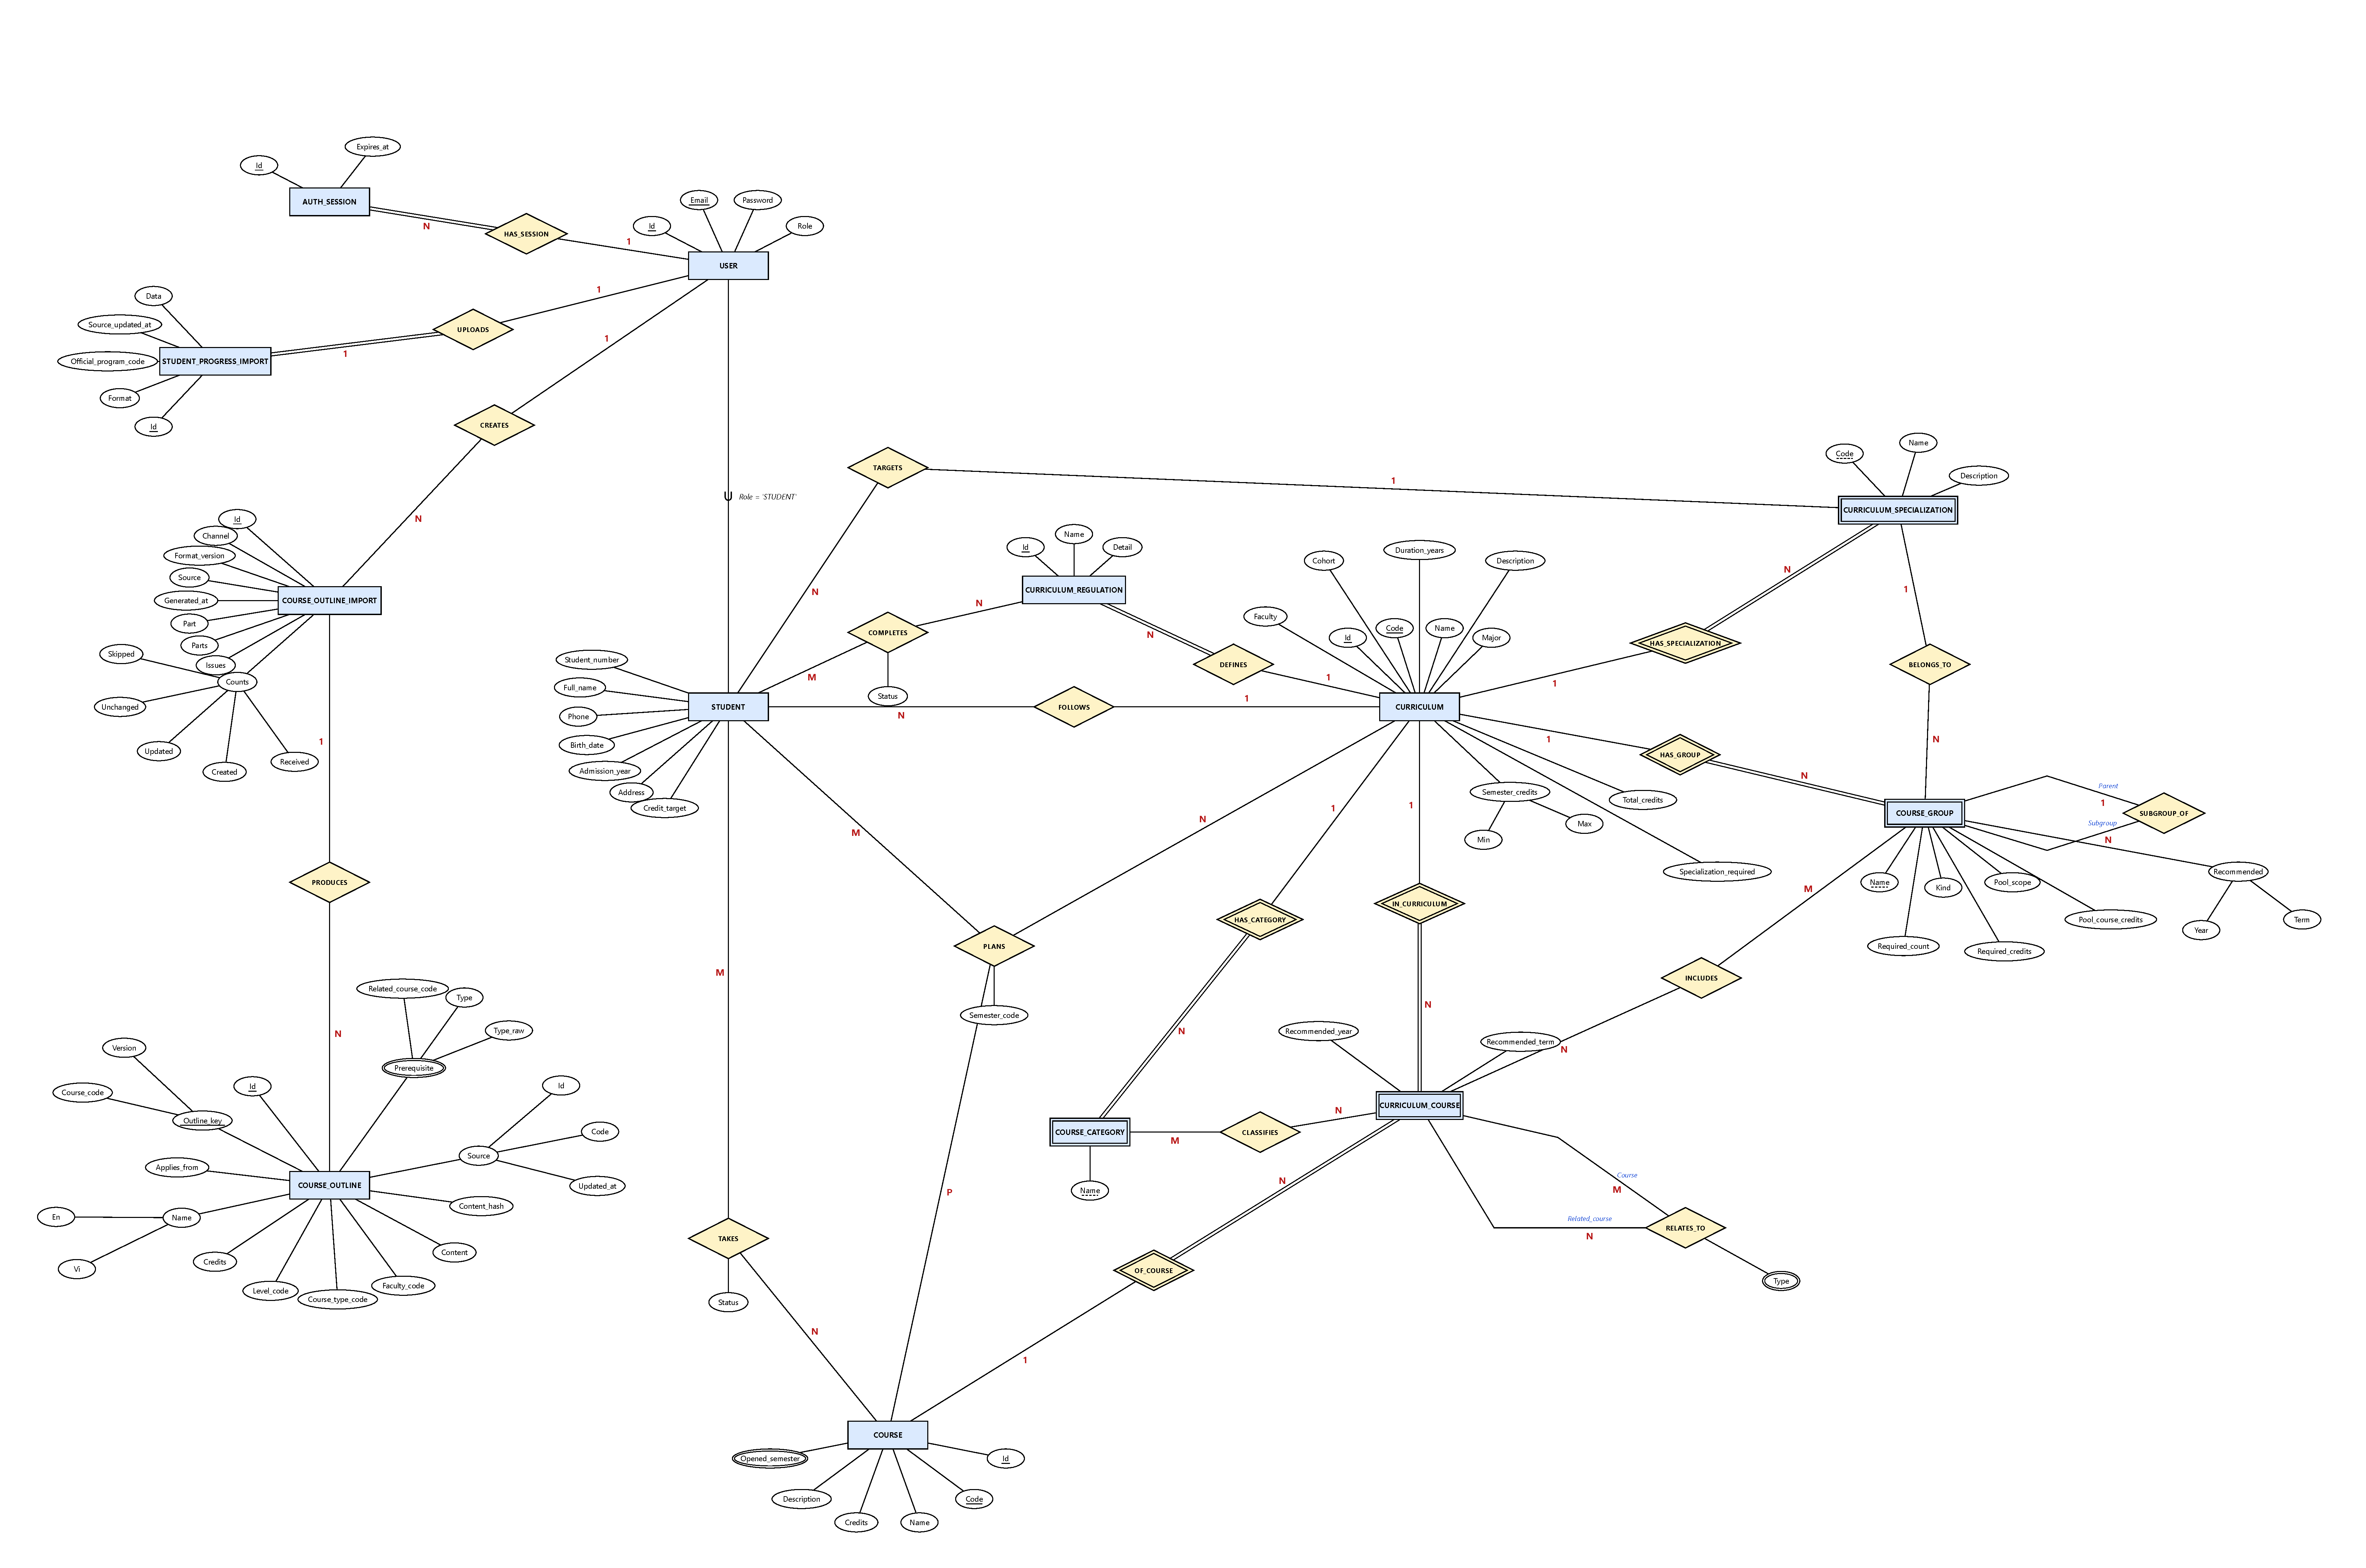
\includegraphics[width=\linewidth,height=0.9\textheight,keepaspectratio]{image/erd-chen.pdf}
        \caption{Entity--relationship diagram of the BK Uni database}
        \label{fig:erd}
    \end{figure}
\end{landscape}
\restoregeometry
\setlength{\headheight}{40pt} % restoregeometry resets the header height set in h_and_d.tex

\subsection{User Interface Designs}
\label{subsec:ui-design}

The final part of the System Design presents the user interface (UI) of BK Uni. As an academic planning assistant for students of Ho Chi Minh City University of Technology, the interface is designed with a strong focus on clarity and on keeping the data that students care about---their curriculum, their course statuses and their progress towards graduation---always one click away. Every student page shares the same layout: a sidebar on the left that groups the functions under \emph{Học tập} (Studying) and \emph{Tài khoản} (Account), a header bar showing the signed-in account, a light/dark theme switch and a sign-out button, and a content area where each page starts with a title, a short explanation of what the page is based on, and its main actions.

At the same time, the UI must stay faithful to the official sources used at the university. Course outlines imported from myBK are shown with the same structure as the original documents, including their version and source, and every figure computed by the system, such as remaining credits or the projected graduation semester, is accompanied by a note explaining how it was derived. In this way, students can trust the information and check it against the university's regulations before registering for courses. The screenshots in this section were captured from the running system using a demo account of a fourth-year Computer Science student (curriculum \texttt{CS-2023-KHMT}, admission year 2023, currently in semester 261).

\subsubsection{Flow Summary}
\label{subsubsec:ui-flow}

To summarize the normal user flow, we present the diagram in Figure~\ref{fig:ui-flow}, showing how a student navigates through BK Uni from signing in to finalizing a study plan. A new student first creates an account on the Register Page and then signs in on the Login Page, after which the system opens the Course List Page. If no curriculum has been selected yet, the pages remind the student to complete the Personal Profile first, since every analysis depends on the curriculum. The student then declares the status and planned semester of each course, opens the Course Detail Page whenever more information about a course is needed, and reviews the overall progress on the Learning Analysis Page. For questions that the analysis alone cannot answer, the student can consult the AI Advisor. Based on what they learn, students return to the Course List Page to adjust their plan, and this loop is repeated until the plan is finalized.

\begin{figure}[H]
    \centering
    \resizebox{!}{0.82\textheight}{%
    \begin{tikzpicture}[
        node distance=0.75cm and 1.1cm,
        font=\small,
        >=stealth,
        box/.style={rectangle, draw, text width=4.4cm, align=center, minimum height=1.1cm, execute at begin node={\hyphenpenalty=10000\relax}},
        term/.style={box, rounded corners=8pt},
        dec/.style={diamond, draw, aspect=2.4, text width=2.7cm, align=center, inner sep=1pt},
        arr/.style={->, thick},
        lbl/.style={font=\footnotesize, fill=white, inner sep=1.5pt}
    ]
        \node[term] (start) {Lands on the \textbf{Login Page}};
        \node[dec, below=of start] (acc) {Has an account?};
        \node[box, left=of acc] (reg) {Creates an account on the \textbf{Register Page}};
        \node[box, below=of acc] (signin) {Signs in with email and password};
        \node[box, below=of signin] (list) {Navigates to the \textbf{Course List Page}};
        \node[dec, below=of list] (cur) {Curriculum selected?};
        \node[box, left=of cur] (prof) {Fills in personal information and selects the curriculum on the \textbf{Personal Profile Page}};
        \node[box, below=of cur] (declare) {Declares course statuses and planned semesters on the \textbf{Course List Page}};
        \node[dec, below=of declare] (det) {Wants to view a course in detail?};
        \node[box, right=of det] (detail) {Views the outline and opening history on the \textbf{Course Detail Page}};
        \node[box, below=of det] (ana) {Reviews progress, missing courses and options on the \textbf{Learning Analysis Page}};
        \node[dec, below=of ana] (adv) {Needs further advice?};
        \node[box, below=of adv] (ai) {Chats with the AI on the \textbf{AI Advisor Page} and checks its \textbf{Trajectory}};
        \node[dec, below=of ai] (fin) {Study plan finalized?};
        \node[term, below=of fin] (end) {End};

        \draw[arr] (start) -- (acc);
        \draw[arr] (acc) -- node[lbl] {Yes} (signin);
        \draw[arr] (acc) -- node[lbl] {No} (reg);
        \draw[arr] (reg) |- (signin);
        \draw[arr] (signin) -- (list);
        \draw[arr] (list) -- (cur);
        \draw[arr] (cur) -- node[lbl] {Yes} (declare);
        \draw[arr] (cur) -- node[lbl] {No} (prof);
        \draw[arr] (prof) |- (list);
        \draw[arr] (declare) -- (det);
        \draw[arr] (det) -- node[lbl] {Yes} (detail);
        \draw[arr] (detail.north) |- ([yshift=-2mm]declare.east);
        \draw[arr] (det) -- node[lbl] {No} (ana);
        \draw[arr] (ana) -- (adv);
        \draw[arr] (adv) -- node[lbl] {Yes} (ai);
        \draw[arr] (adv.west) -- node[lbl, pos=0.5] {No} ++(-1.4,0) |- (fin.west);
        \draw[arr] (ai) -- (fin);
        \draw[arr] (fin) -- node[lbl] {Yes} (end);
        \draw[arr] (fin.east) -- node[lbl, pos=0.12] {No} ($(fin.east -| detail.east)+(0.8,0)$) |- ([yshift=2mm]declare.east);
    \end{tikzpicture}%
    }
    \caption{UI flow of a student in BK Uni}
    \label{fig:ui-flow}
\end{figure}

In the following subsections, the main pages of this flow are described in turn, together with the design decisions behind them.

\subsubsection{Course List Page}
\label{subsubsec:ui-course-list}

After signing in, students land on the \emph{Môn học \& kế hoạch} (Courses \& Plan) page, shown in Figure~\ref{fig:ui-courses}. To give an overview at a glance, the top of the page contains four summary cards: the number of courses the student has declared, the number of completed courses over the number of required ones, the accumulated credits over the credits required for graduation, and the credits already placed in the study plan. Below them, the \emph{Kế hoạch theo học kỳ} (Plan by semester) card groups the planned courses by the semester in which the student intends to take them.

\begin{figure}[H]
    \centering
    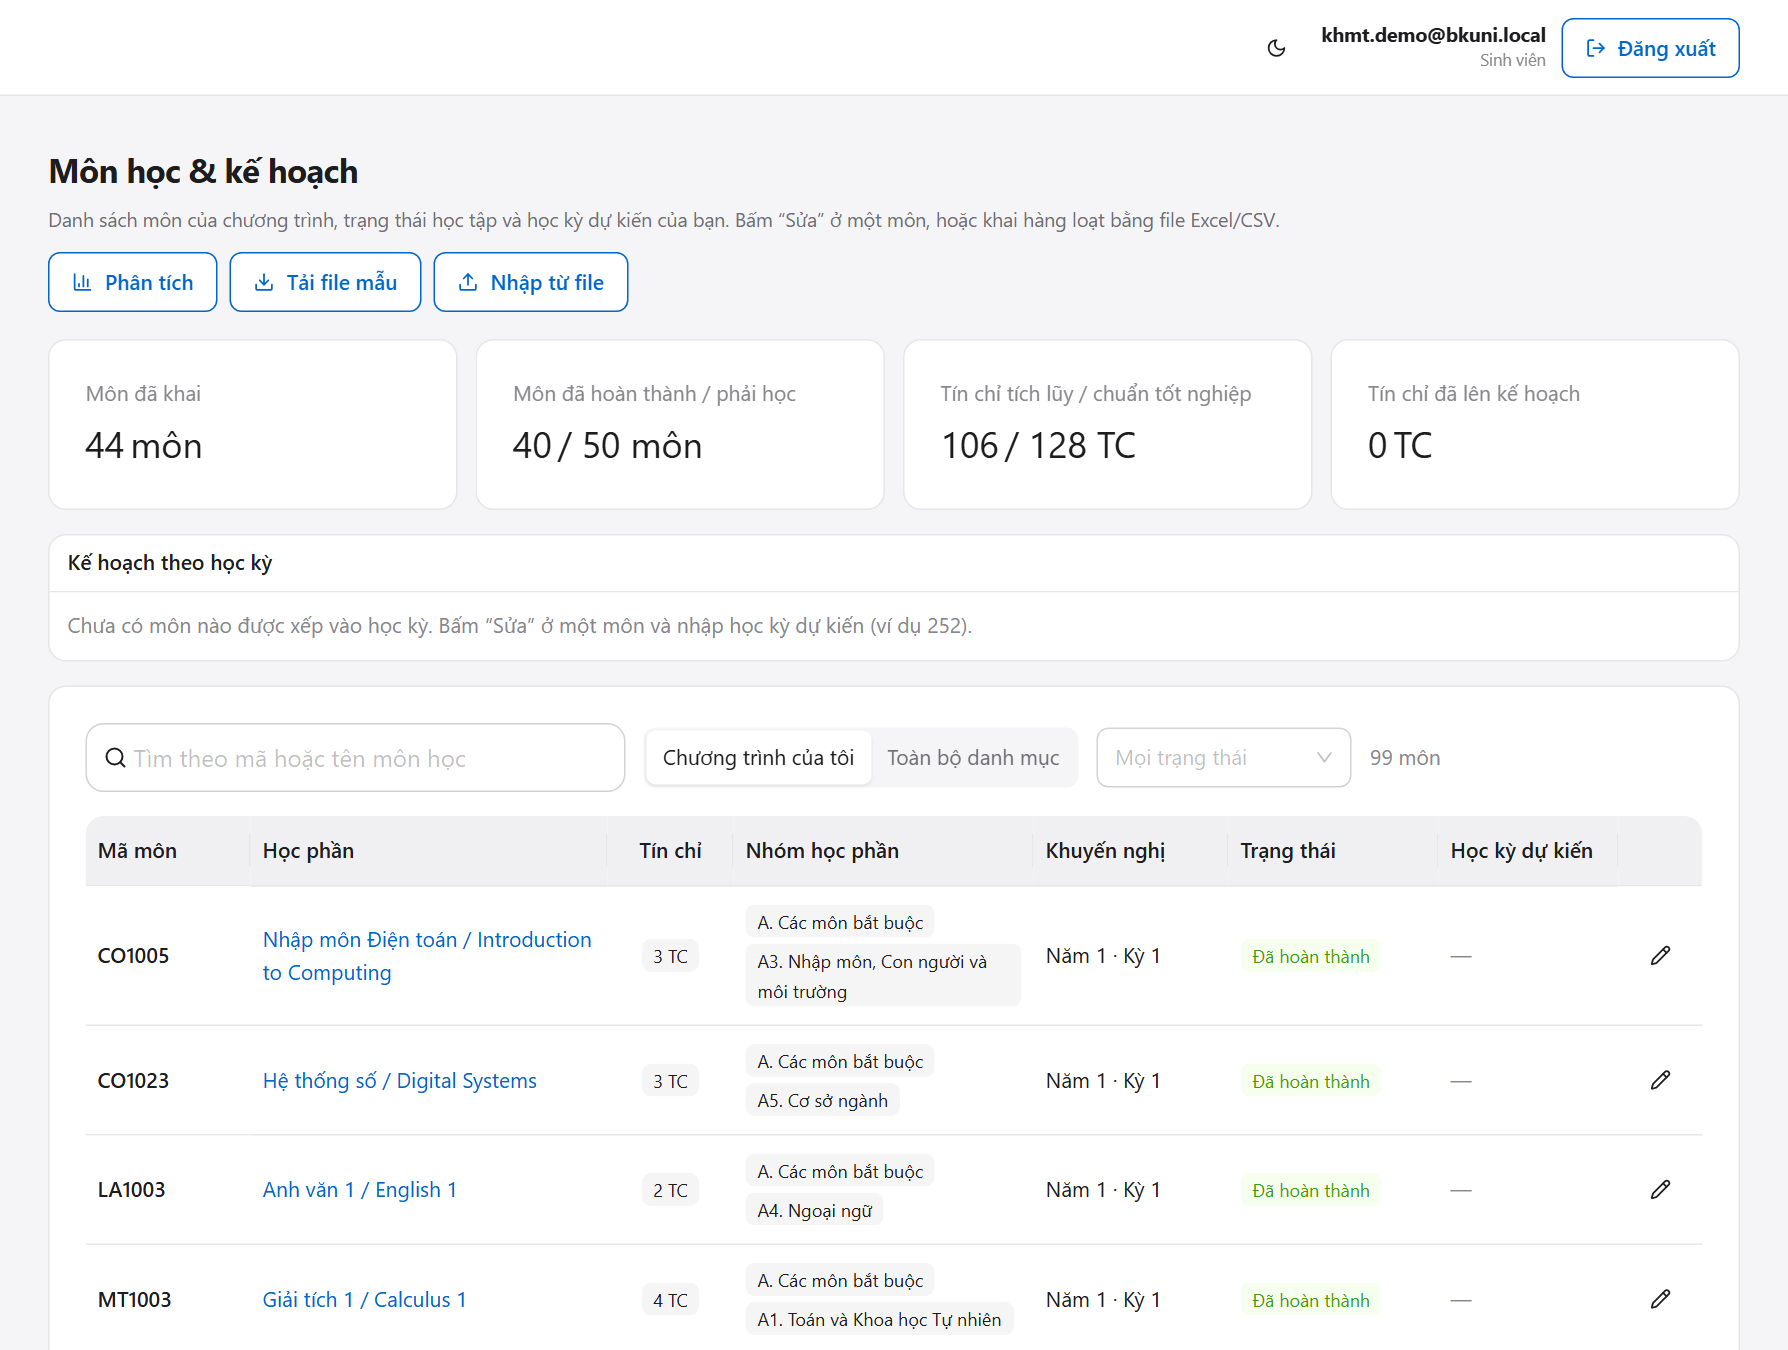
\includegraphics[width=\textwidth]{image/ui/courses.png}
    \caption{The Course List page}
    \label{fig:ui-courses}
\end{figure}

The main part of the page is the course table. Students can search by course code or name, switch between the courses of their own curriculum and the whole course catalog, and filter by learning status. Each row shows the course code and name, the number of credits, the course groups it belongs to, the recommended year and term according to the curriculum, the current status and the planned semester. Clicking the pencil icon at the end of a row lets the student update the status and planned semester of a single course, while the \emph{Tải file mẫu} (Download template) and \emph{Nhập từ file} (Import from file) buttons allow declaring many courses at once through an Excel/CSV file. The \emph{Phân tích} (Analysis) button leads to the Learning Analysis page described in Section~\ref{subsubsec:ui-analysis}.

\subsubsection{Course Detail Page}
\label{subsubsec:ui-course-detail}

Selecting a course name in the table navigates the student to the Course Detail page. The page is divided into two cards. The upper card summarizes the course within the student's curriculum: its code, name, credits, course groups, the student's own learning status and the time it was last updated. The lower card, \emph{Đề cương môn học} (Course outline), displays the outline imported from myBK. Its header contains a switch between Vietnamese and English and a selector of outline versions, in which the version that applies to the current semester is marked as \emph{Đang áp dụng} (In effect). Under the header, the general information of the outline---faculty, department, level, course type and knowledge block---is listed together with the source document and its update date. The content of the outline is then organized into six tabs so that students can jump directly to the part they need. Figure~\ref{fig:ui-detail-intro} shows the page with the first tab, \emph{Giới thiệu} (Introduction), opened for the course \texttt{CO1005}; this tab presents the course objectives, a short summary, study guidelines and the list of textbooks and references.

\begin{figure}[H]
    \centering
    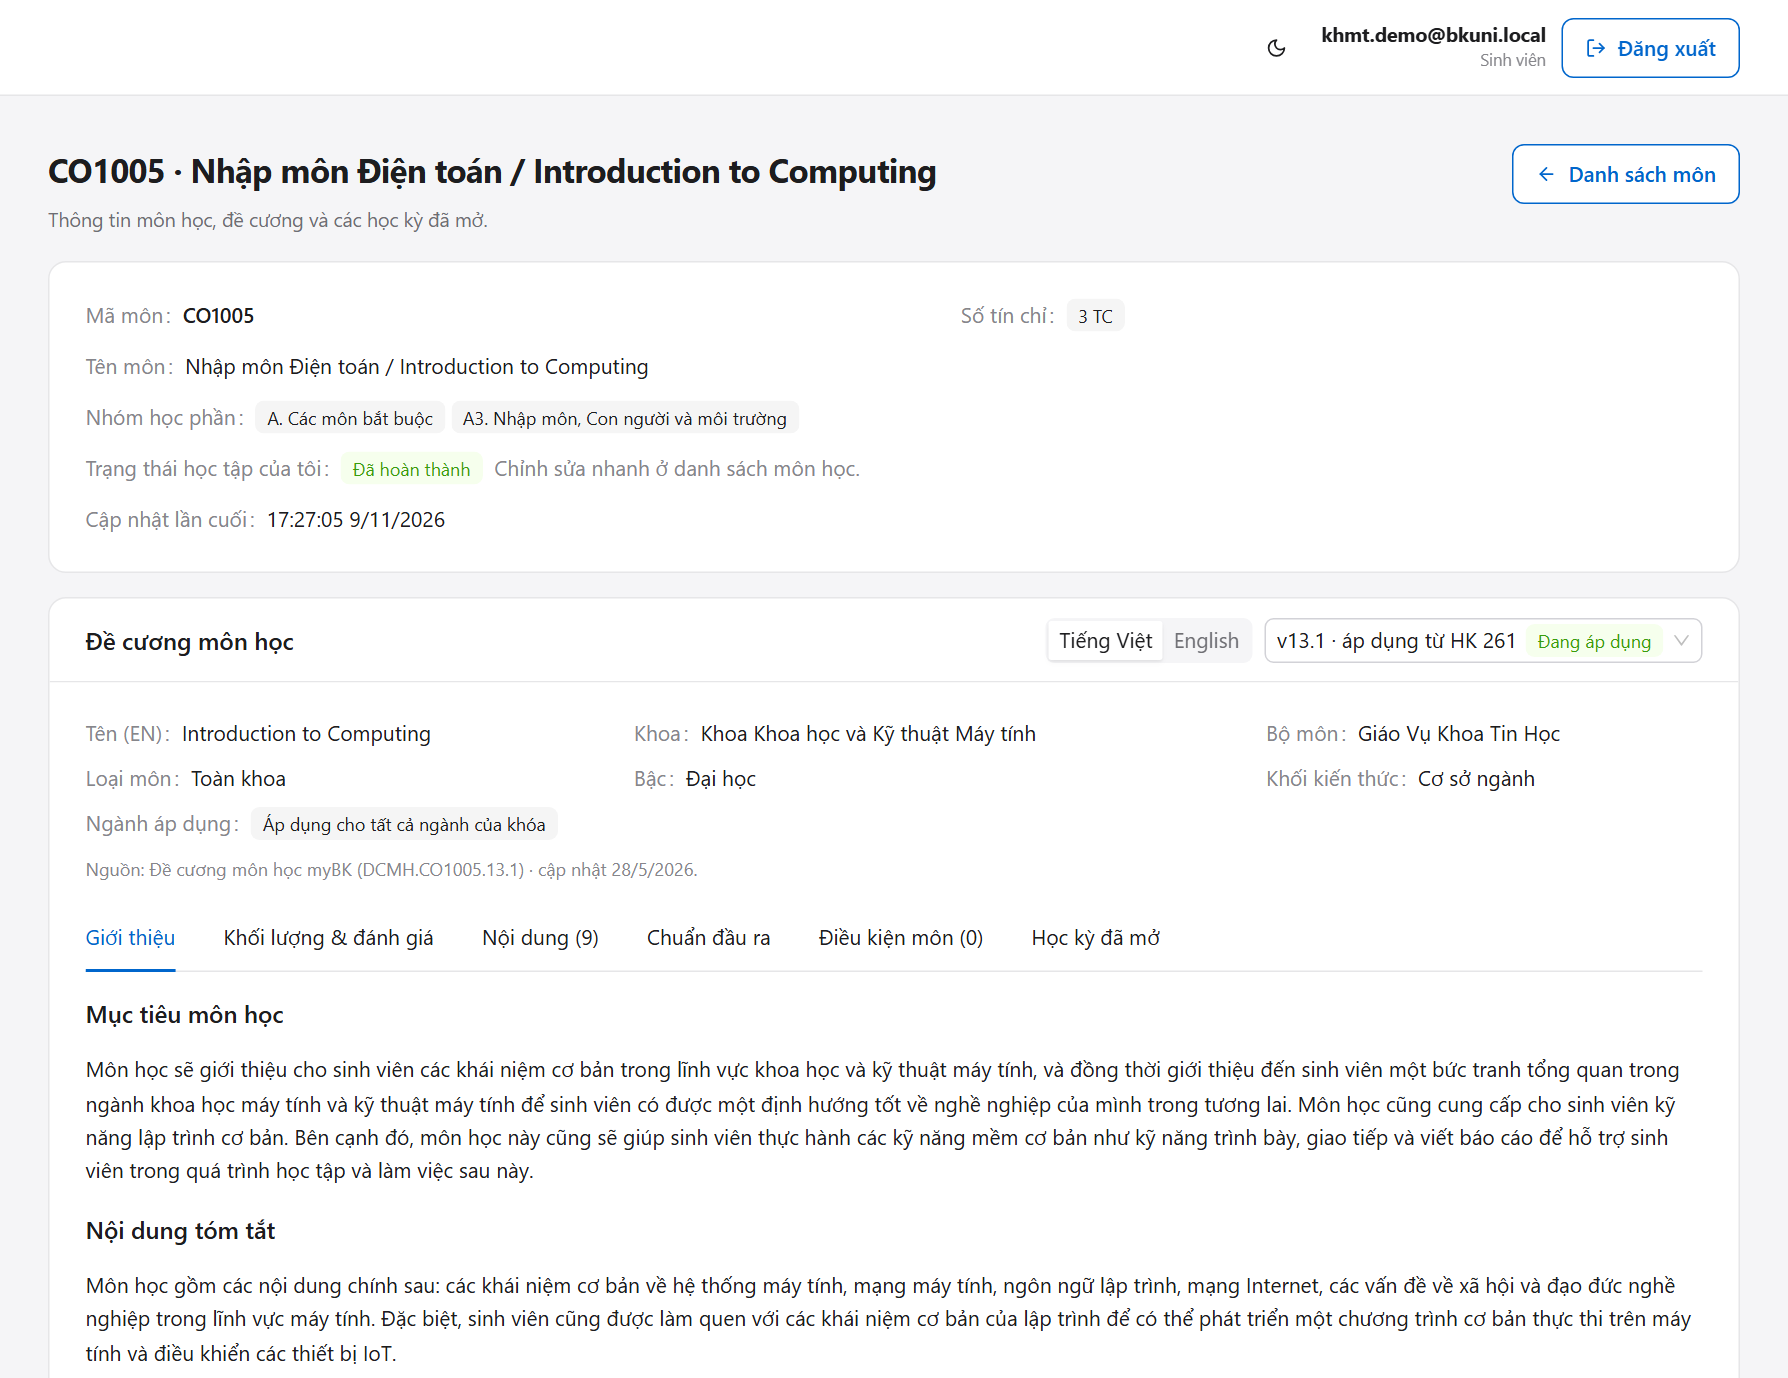
\includegraphics[width=\textwidth]{image/ui/detail-intro.png}
    \caption{The Course Detail page with the Introduction tab}
    \label{fig:ui-detail-intro}
\end{figure}

The \emph{Khối lượng \& đánh giá} (Workload \& Assessment) tab, shown in Figure~\ref{fig:ui-detail-workload}, turns the numbers in the outline into simple bar charts. On the left, the grading scheme shows the weight of each assessment component together with the format and duration of the midterm and final exams. On the right, the study workload shows the total number of periods, the estimated study hours and ECTS credits, and the breakdown into theory, laboratory, assignments, self-study and other activities. This helps students estimate how demanding a course is before choosing it.

\begin{figure}[H]
    \centering
    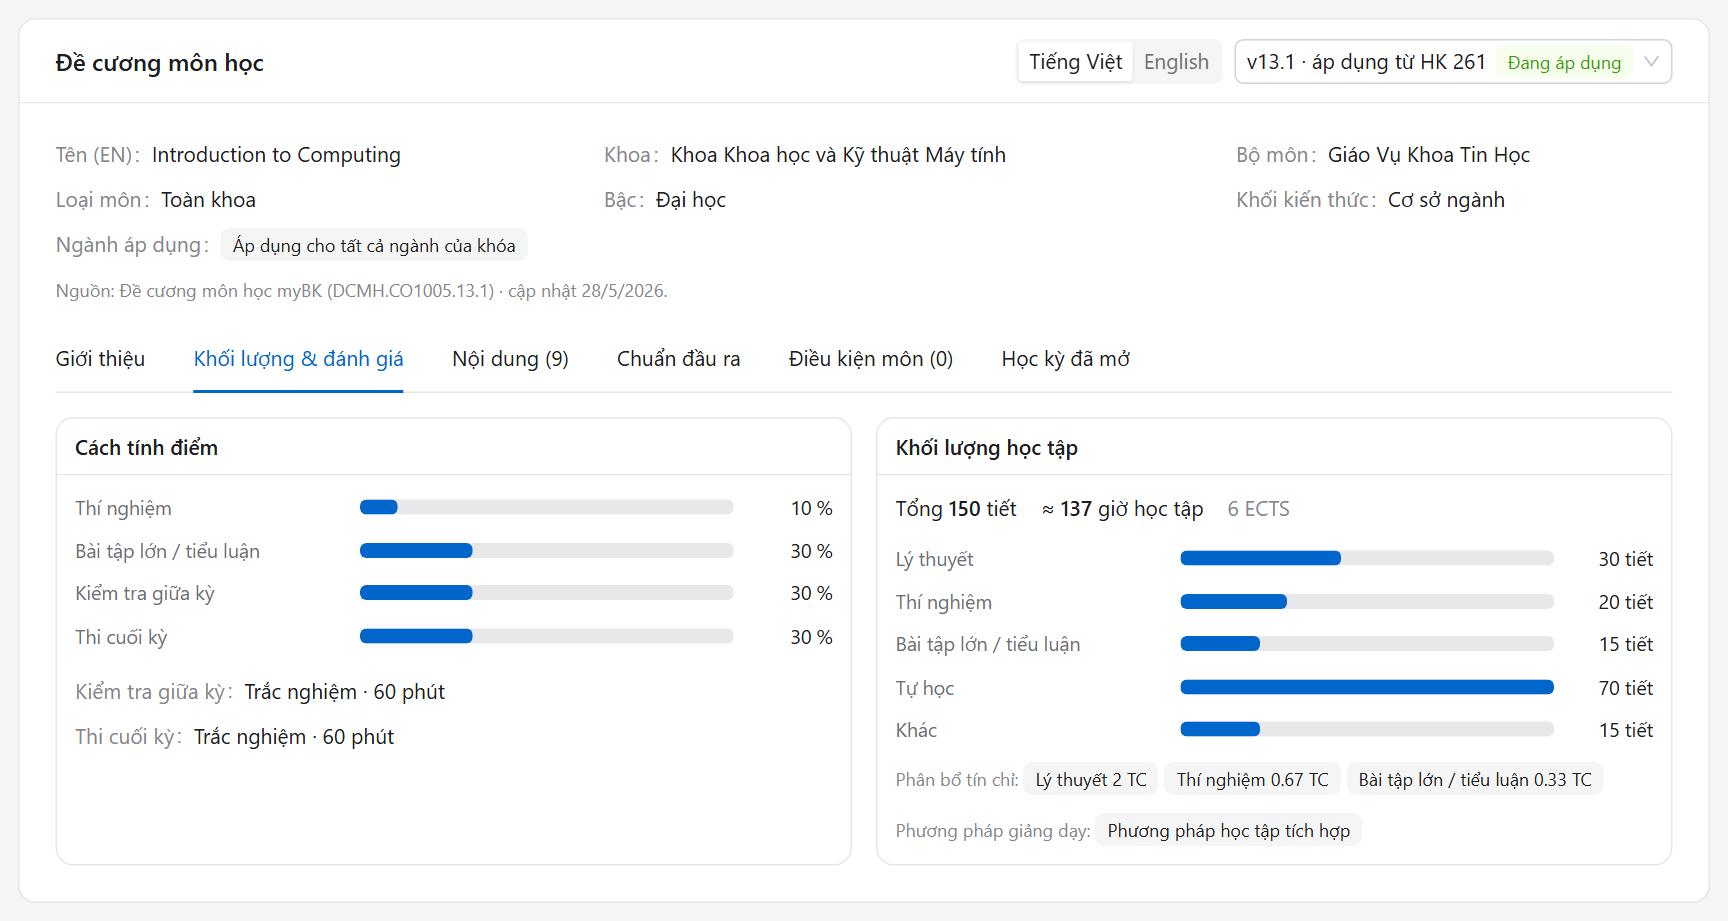
\includegraphics[width=0.9\textwidth]{image/ui/detail-workload.png}
    \caption{The Workload \& Assessment tab}
    \label{fig:ui-detail-workload}
\end{figure}

The \emph{Nội dung} (Content) tab, illustrated in Figure~\ref{fig:ui-detail-sessions}, lists the teaching sessions of the course in order; the number in the tab label indicates the number of session blocks. Each block shows the range of sessions it covers, the topics taught, the activities expected from students, and two kinds of tags: blue tags for the learning outcomes achieved in the block and yellow tags for the related assessment activities. Hovering over a tag reveals its full description.

\begin{figure}[H]
    \centering
    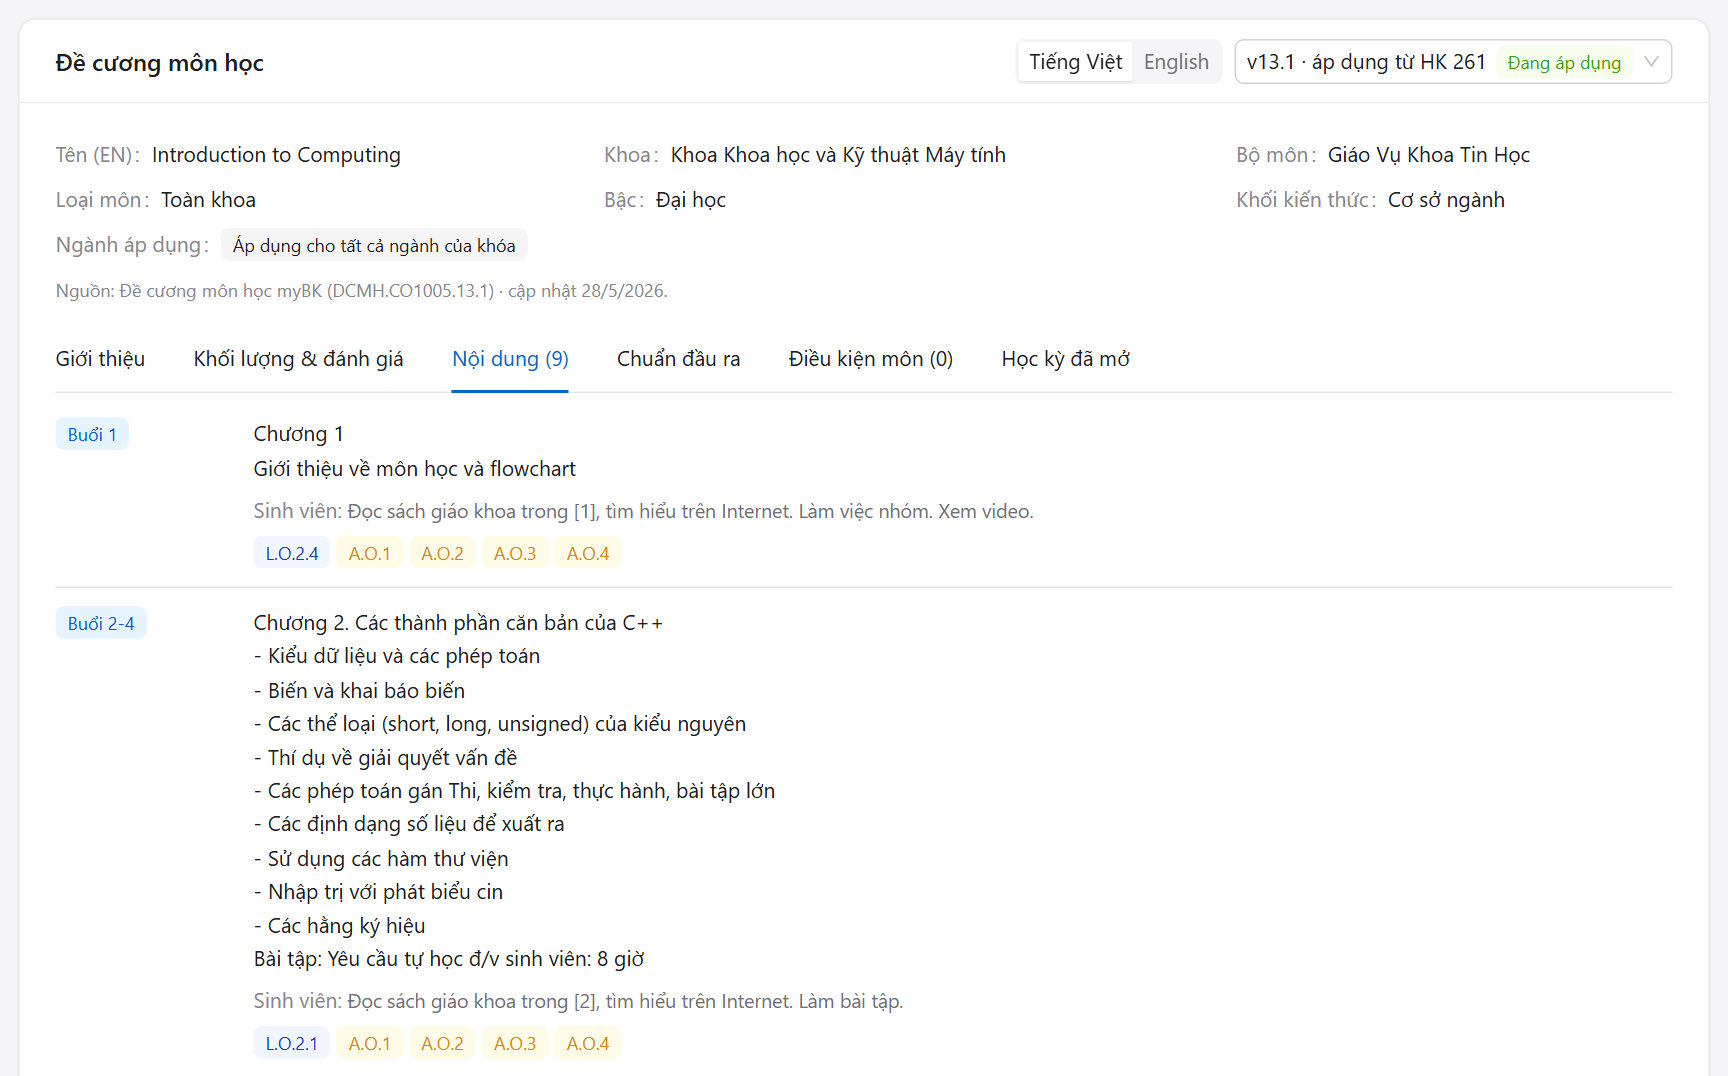
\includegraphics[width=0.9\textwidth]{image/ui/detail-sessions.png}
    \caption{The Content tab listing the teaching sessions}
    \label{fig:ui-detail-sessions}
\end{figure}

The \emph{Chuẩn đầu ra} (Learning Outcomes) tab, shown in Figure~\ref{fig:ui-detail-outcomes}, presents the learning outcomes of the course as a hierarchy, in which each detailed outcome is linked to the assessment activities used to evaluate it. The list of assessment activities and their corresponding forms of evaluation is given at the bottom of the tab.

\begin{figure}[H]
    \centering
    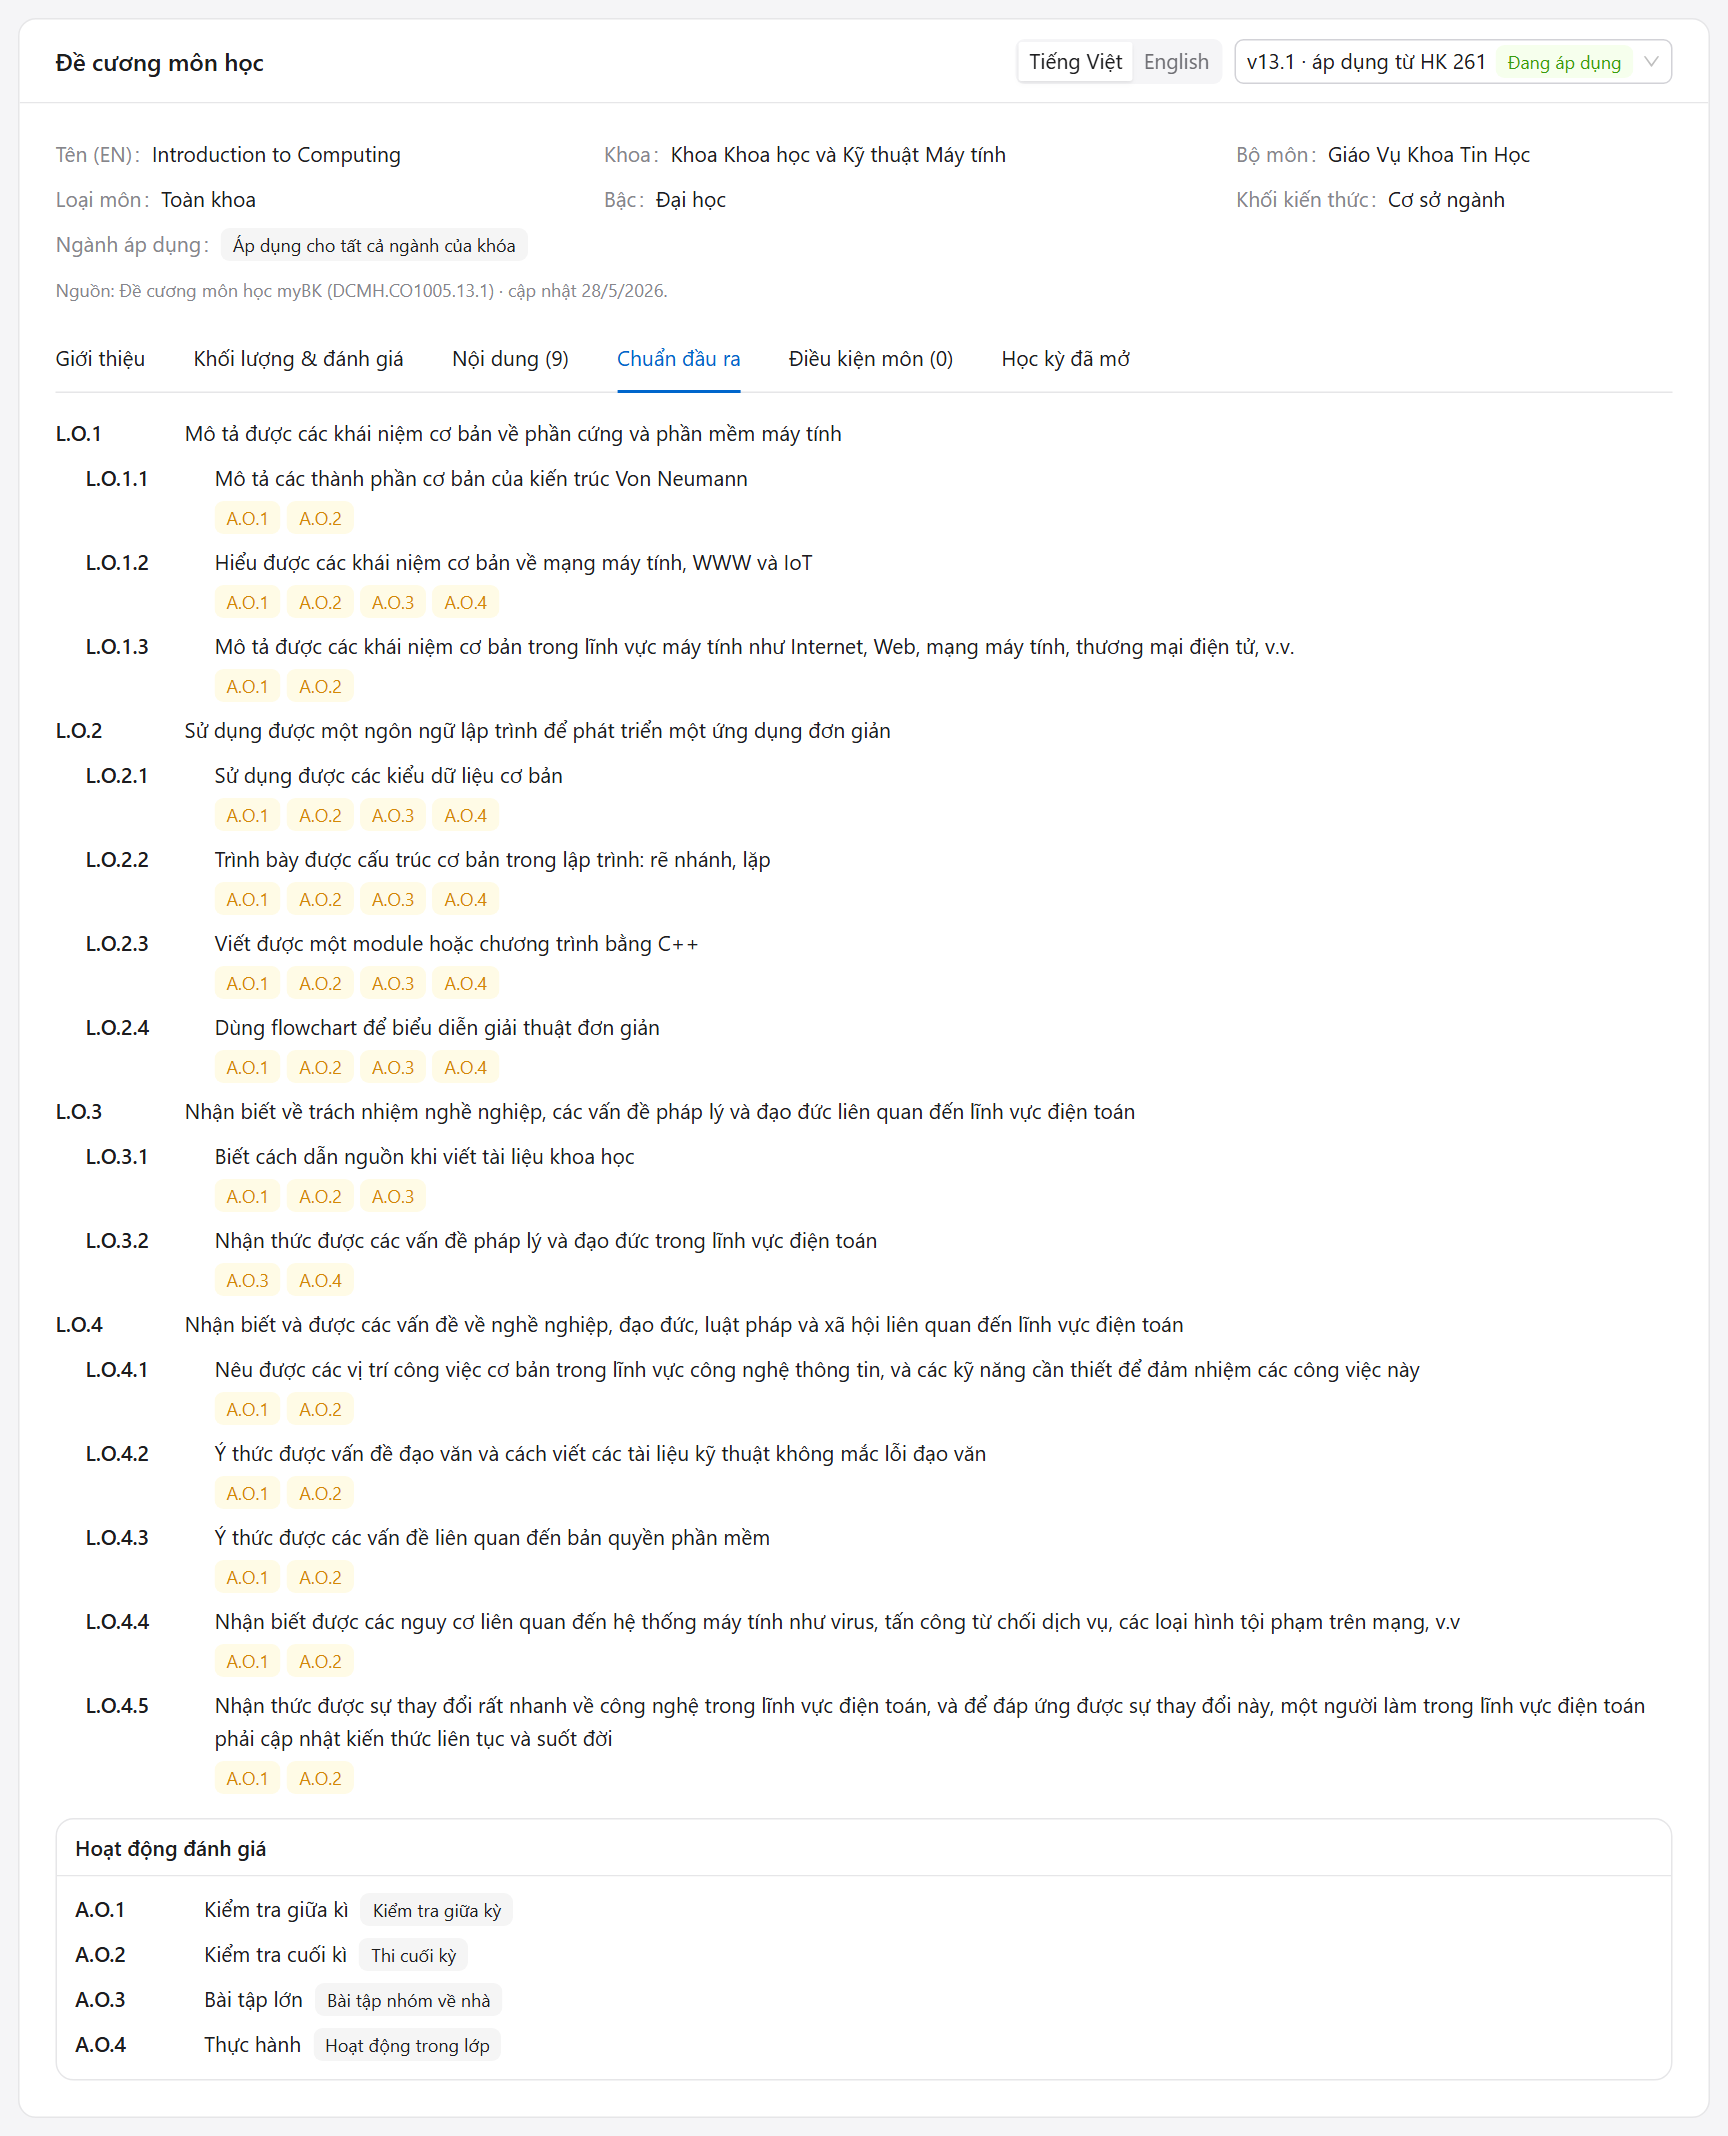
\includegraphics[width=0.9\textwidth,height=0.75\textheight,keepaspectratio]{image/ui/detail-outcomes.png}
    \caption{The Learning Outcomes tab}
    \label{fig:ui-detail-outcomes}
\end{figure}

Finally, the \emph{Học kỳ đã mở} (Opened Semesters) tab, shown in Figure~\ref{fig:ui-detail-opened}, helps students predict whether a course will be offered in the coming semesters. The history is drawn as a grid in which each row is an academic year and each column is a term (first term, second term and summer term). Each cell indicates whether the course was opened, not opened, or has not yet taken place, and the current semester is highlighted with a dark border. Below the grid, a frequency bar summarizes how often the course was opened in each term, followed by a short conclusion in plain language.

\begin{figure}[H]
    \centering
    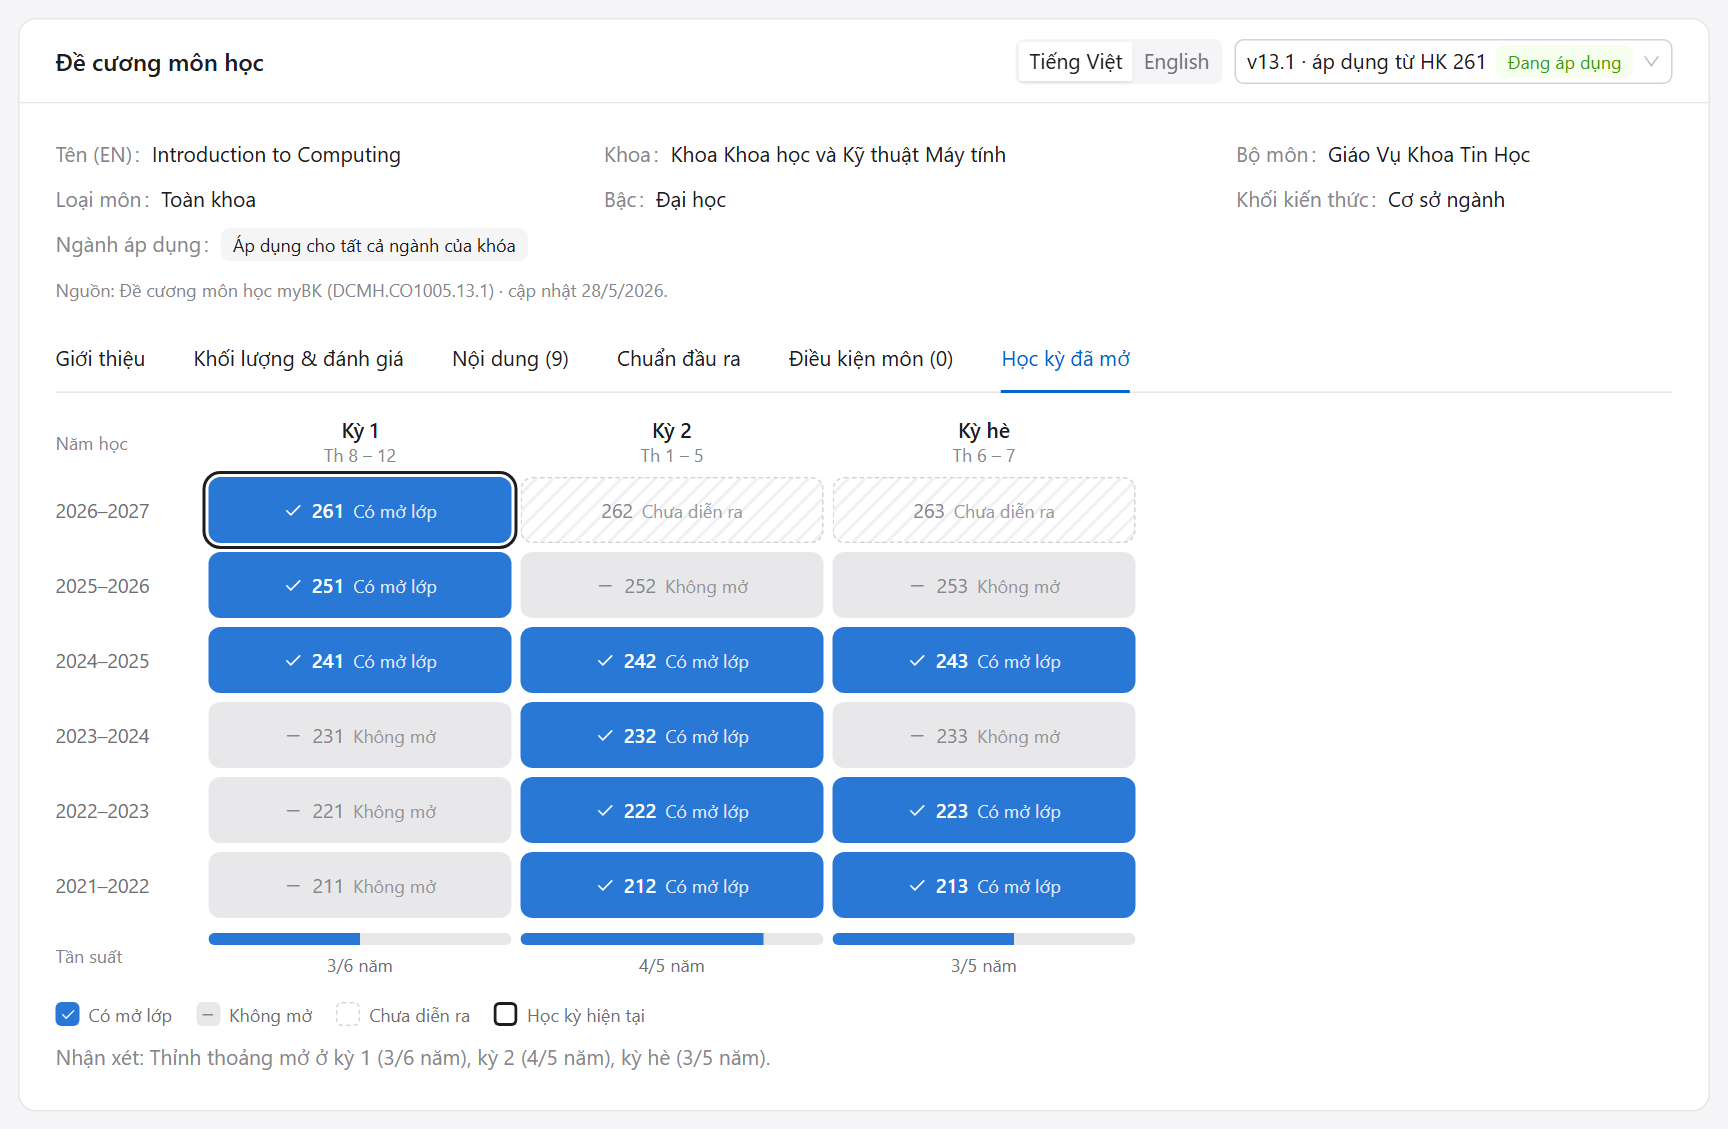
\includegraphics[width=0.9\textwidth]{image/ui/detail-opened.png}
    \caption{The Opened Semesters tab}
    \label{fig:ui-detail-opened}
\end{figure}

\subsubsection{Learning Analysis Page}
\label{subsubsec:ui-analysis}

From the Course List page, students can open the \emph{Phân tích học tập} (Learning Analysis) page, which combines the curriculum, the declared course statuses and the study plan to evaluate the student's progress towards graduation. The subtitle of the page states exactly which curriculum and which semester the analysis is based on, as well as how many courses have an outline available. The content of the page is organized into a series of cards, each answering one question about the student's progress; the main ones are presented below.

At the top of the page, the overview card shown in Figure~\ref{fig:ui-analysis-overview} answers the question of how far the student is from graduation. A ring chart shows the percentage of graduation credits earned, next to the number of earned credits over the required credits and the number of courses counted towards graduation. On the right are the key figures: credits in progress, credits planned, credits still missing, the average number of credits completed per semester so far, the number of credits per semester required to graduate on time, and the projected graduation semester compared with the standard one. A stacked bar at the bottom of the card splits the graduation credits into completed, in-progress, planned and missing parts.

\begin{figure}[H]
    \centering
    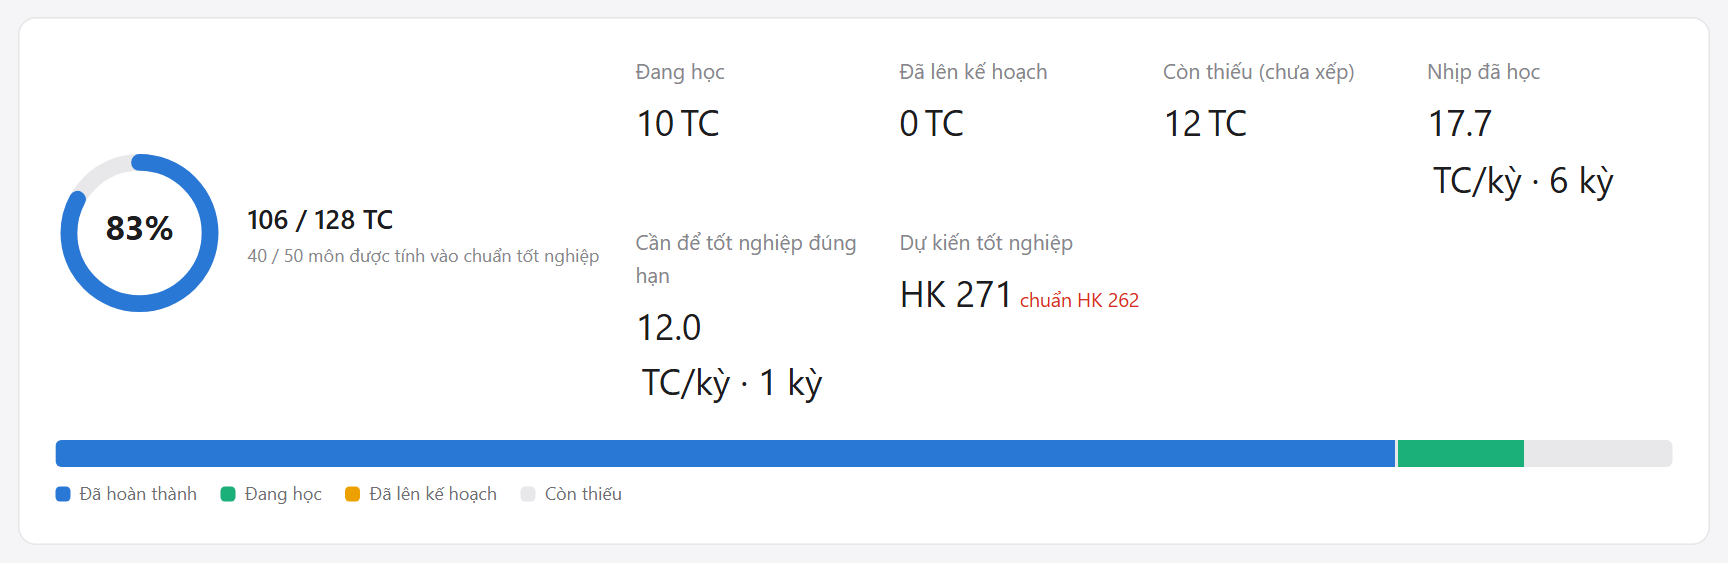
\includegraphics[width=\textwidth]{image/ui/analysis-overview.png}
    \caption{The overview card of the Learning Analysis page}
    \label{fig:ui-analysis-overview}
\end{figure}

Below the overview, two charts placed side by side break the progress down further, as shown in Figure~\ref{fig:ui-analysis-progress}. On the left, \emph{Tiến độ theo khối kiến thức} (Progress by knowledge block) shows one progress bar for the required courses and for each elective group, together with the number of courses that must be chosen in the group. On the right, \emph{Theo khung chương trình (môn bắt buộc)} (By curriculum framework, required courses) is a column chart in which each column is a semester of the standard framework, mapped to the actual semester according to the admission year. The column of the current semester is highlighted with a background, and grey parts in the earlier columns reveal required courses that the student is behind on.

\begin{figure}[H]
    \centering
    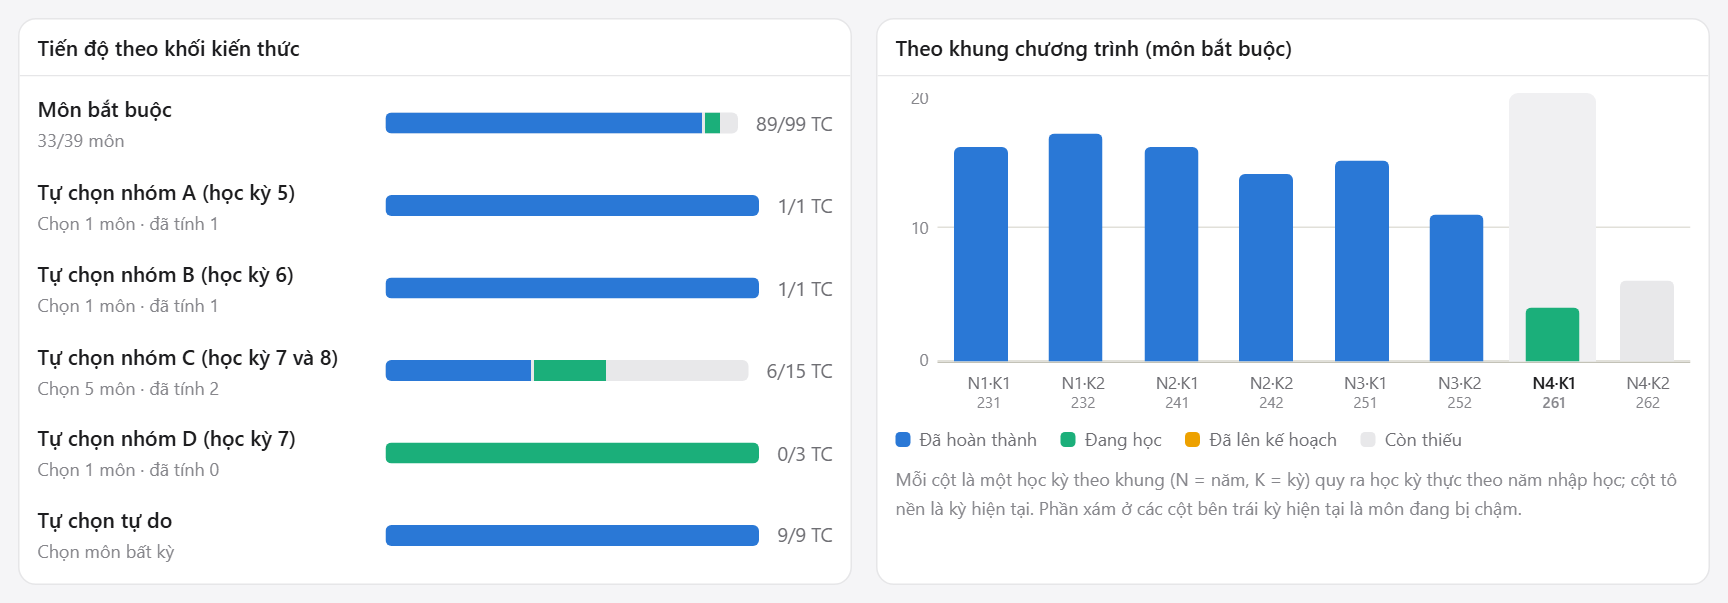
\includegraphics[width=\textwidth]{image/ui/analysis-progress.png}
    \caption{Progress by knowledge block and by curriculum framework}
    \label{fig:ui-analysis-progress}
\end{figure}

The \emph{Môn còn thiếu} (Missing courses) card, shown in Figure~\ref{fig:ui-analysis-missing}, lists the courses that the student still has to complete, grouped into four tabs: required courses whose recommended semester has already passed, the remaining required courses, the elective groups that still lack courses, and the courses that the student has failed. The figure shows the \emph{Bắt buộc còn lại} (Remaining required courses) tab, which contains four courses for the demo student. Each row gives the course name together with its exam format and estimated study hours, its credits and recommended semester, whether the student meets its requirements, how often it has been opened in the next term along with the latest semester it was opened, and the student's current status. When the outline states an additional requirement that is not declared in the curriculum, such as the prerequisite \texttt{CO4359} of the capstone project \texttt{CO4337}, it is highlighted in orange next to the eligibility tag so that the student can verify it with the faculty.

\begin{figure}[H]
    \centering
    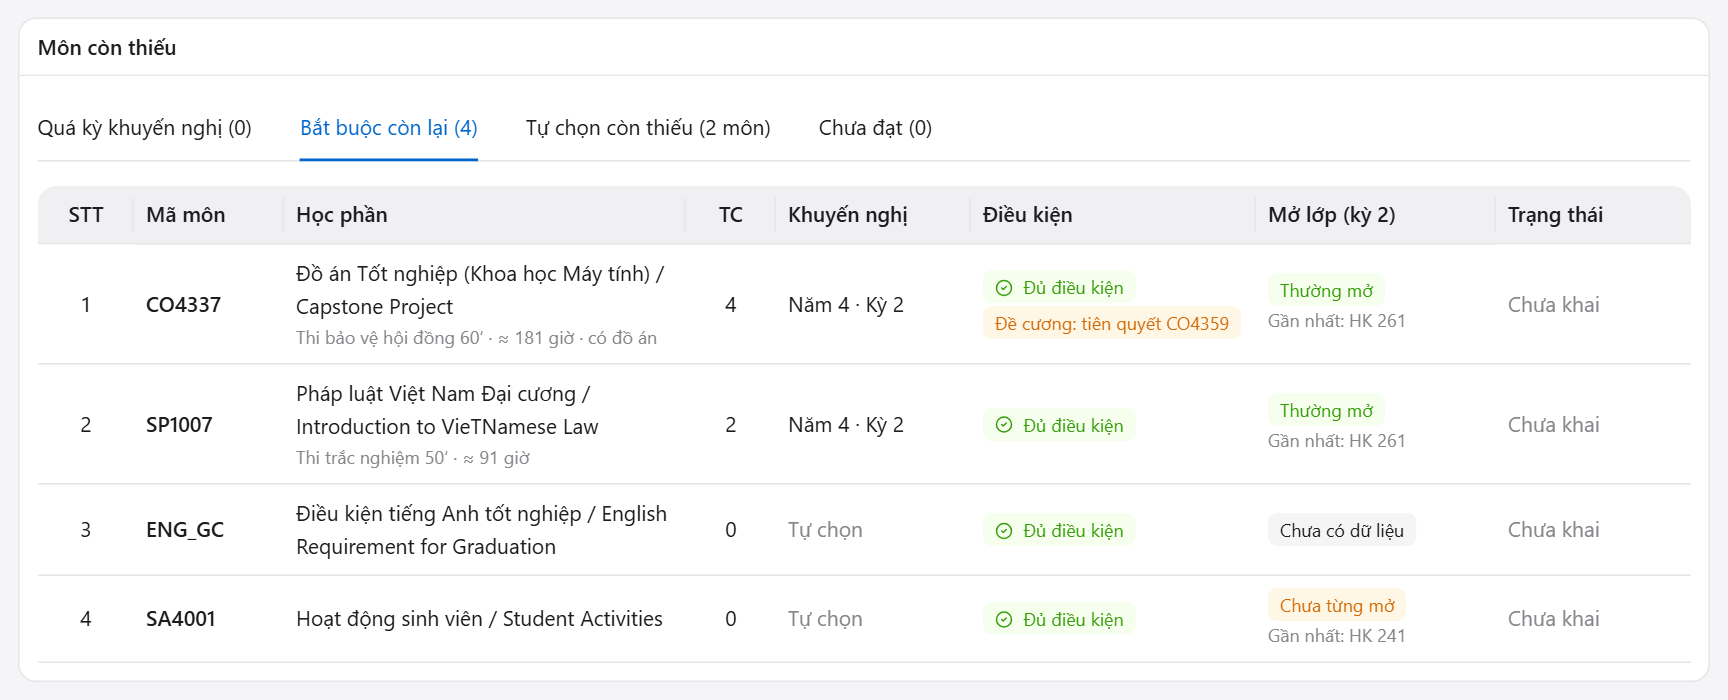
\includegraphics[width=\textwidth]{image/ui/analysis-missing.png}
    \caption{The Missing courses card}
    \label{fig:ui-analysis-missing}
\end{figure}

The \emph{Các lựa chọn} (Options) card, illustrated in Figure~\ref{fig:ui-analysis-options}, supports the student in choosing a specialization and electives. Its first part, \emph{Chuyên ngành (không bắt buộc)} (Specializations, optional), shows one progress bar per specialization, counting the courses of its list that the student has taken or is taking. Under each specialization name, a note tells the student whether the specialization is still achievable or, if not, which elective courses outside the list prevent it. The second part lists, for each elective group that is not yet complete, all candidate courses in a table with their exam format and estimated study hours, the specializations they belong to, their credits, whether the student meets their requirements, how often they are opened in the next term and the student's current status. The figure shows the beginning of the table for elective group C.

\begin{figure}[H]
    \centering
    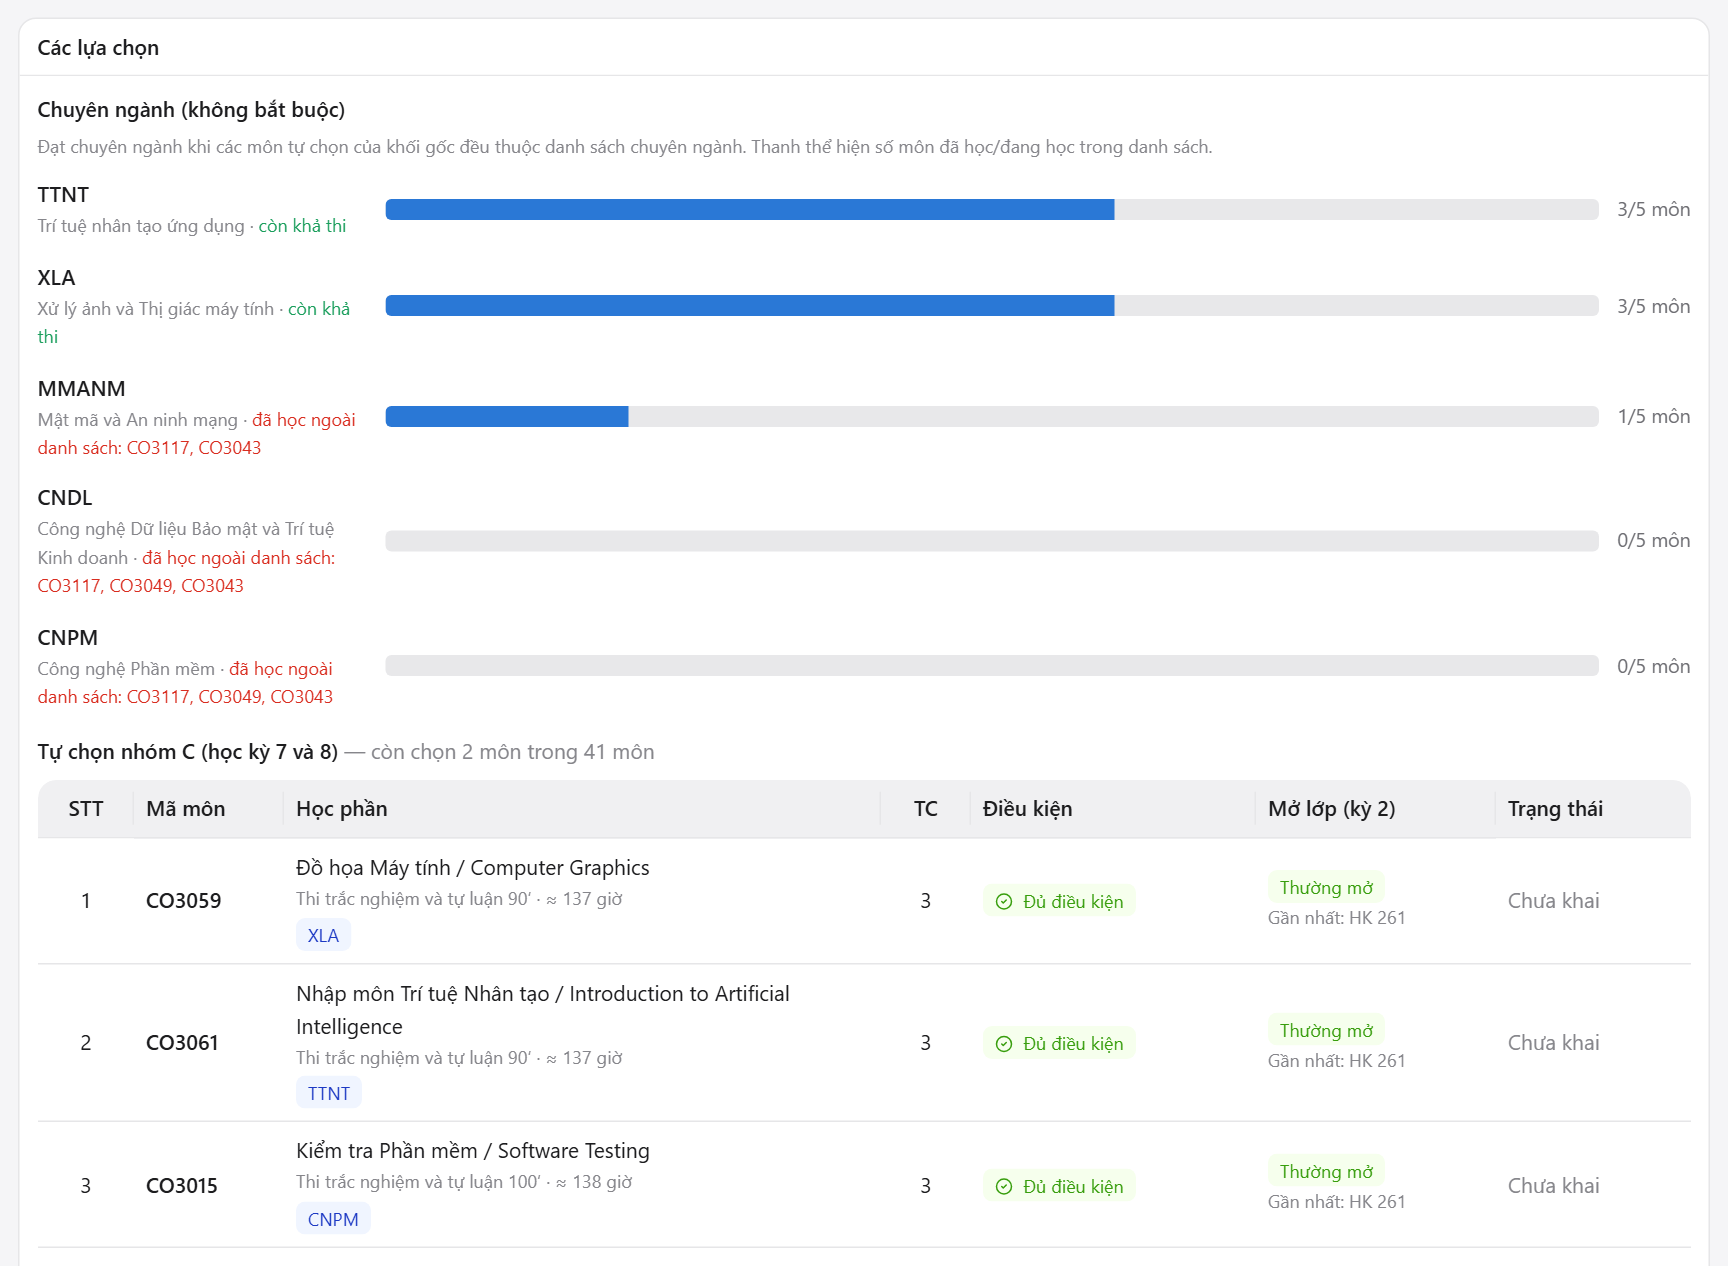
\includegraphics[width=\textwidth]{image/ui/analysis-options.png}
    \caption{The Options card with specializations and elective courses}
    \label{fig:ui-analysis-options}
\end{figure}

Further down, the page also lists the courses that can be registered in the next semester, the ``bottleneck'' courses that unlock the largest number of other courses, and a suggested roadmap to graduation. Finally, the \emph{Điều kiện tốt nghiệp khác} (Other graduation requirements) card, shown in Figure~\ref{fig:ui-analysis-regulations}, reminds the student of the graduation requirements that are not courses, such as the English proficiency requirement and student activities. Each requirement is displayed with an icon indicating whether it has been fulfilled, and the \emph{Cập nhật} (Update) link leads to the graduation regulations page, where the student can update their status.

\begin{figure}[H]
    \centering
    
\includegraphics[width=\textwidth]{image/ui/analysis-regulations.png}
    \caption{The Other graduation requirements card}
    \label{fig:ui-analysis-regulations}
\end{figure}

\subsubsection{AI Advisor Page}
\label{subsubsec:ui-advisor}

For questions that cannot be answered by the analysis alone, such as which elective suits the student's interests, students can turn to the \emph{Tư vấn với AI} (AI Advisor) page. The subtitle reminds students that the advisor relies on the result of the Learning Analysis at the current semester, gives suggestions for the next one, and may be wrong. The header also contains a selector of previous conversations, a \emph{Mới} (New) button to start a new conversation and a \emph{Xóa} (Delete) button. The content area has two tabs: \emph{Trò chuyện} (Chat) and \emph{Trajectory}.

When a new conversation is started, the Chat tab shows a short introduction explaining what the advisor can do, together with several suggested questions so that students can start with one click, as shown in Figure~\ref{fig:ui-advisor-empty}. Questions can also be typed into the input box at the bottom of the page.

\begin{figure}[H]
    \centering
    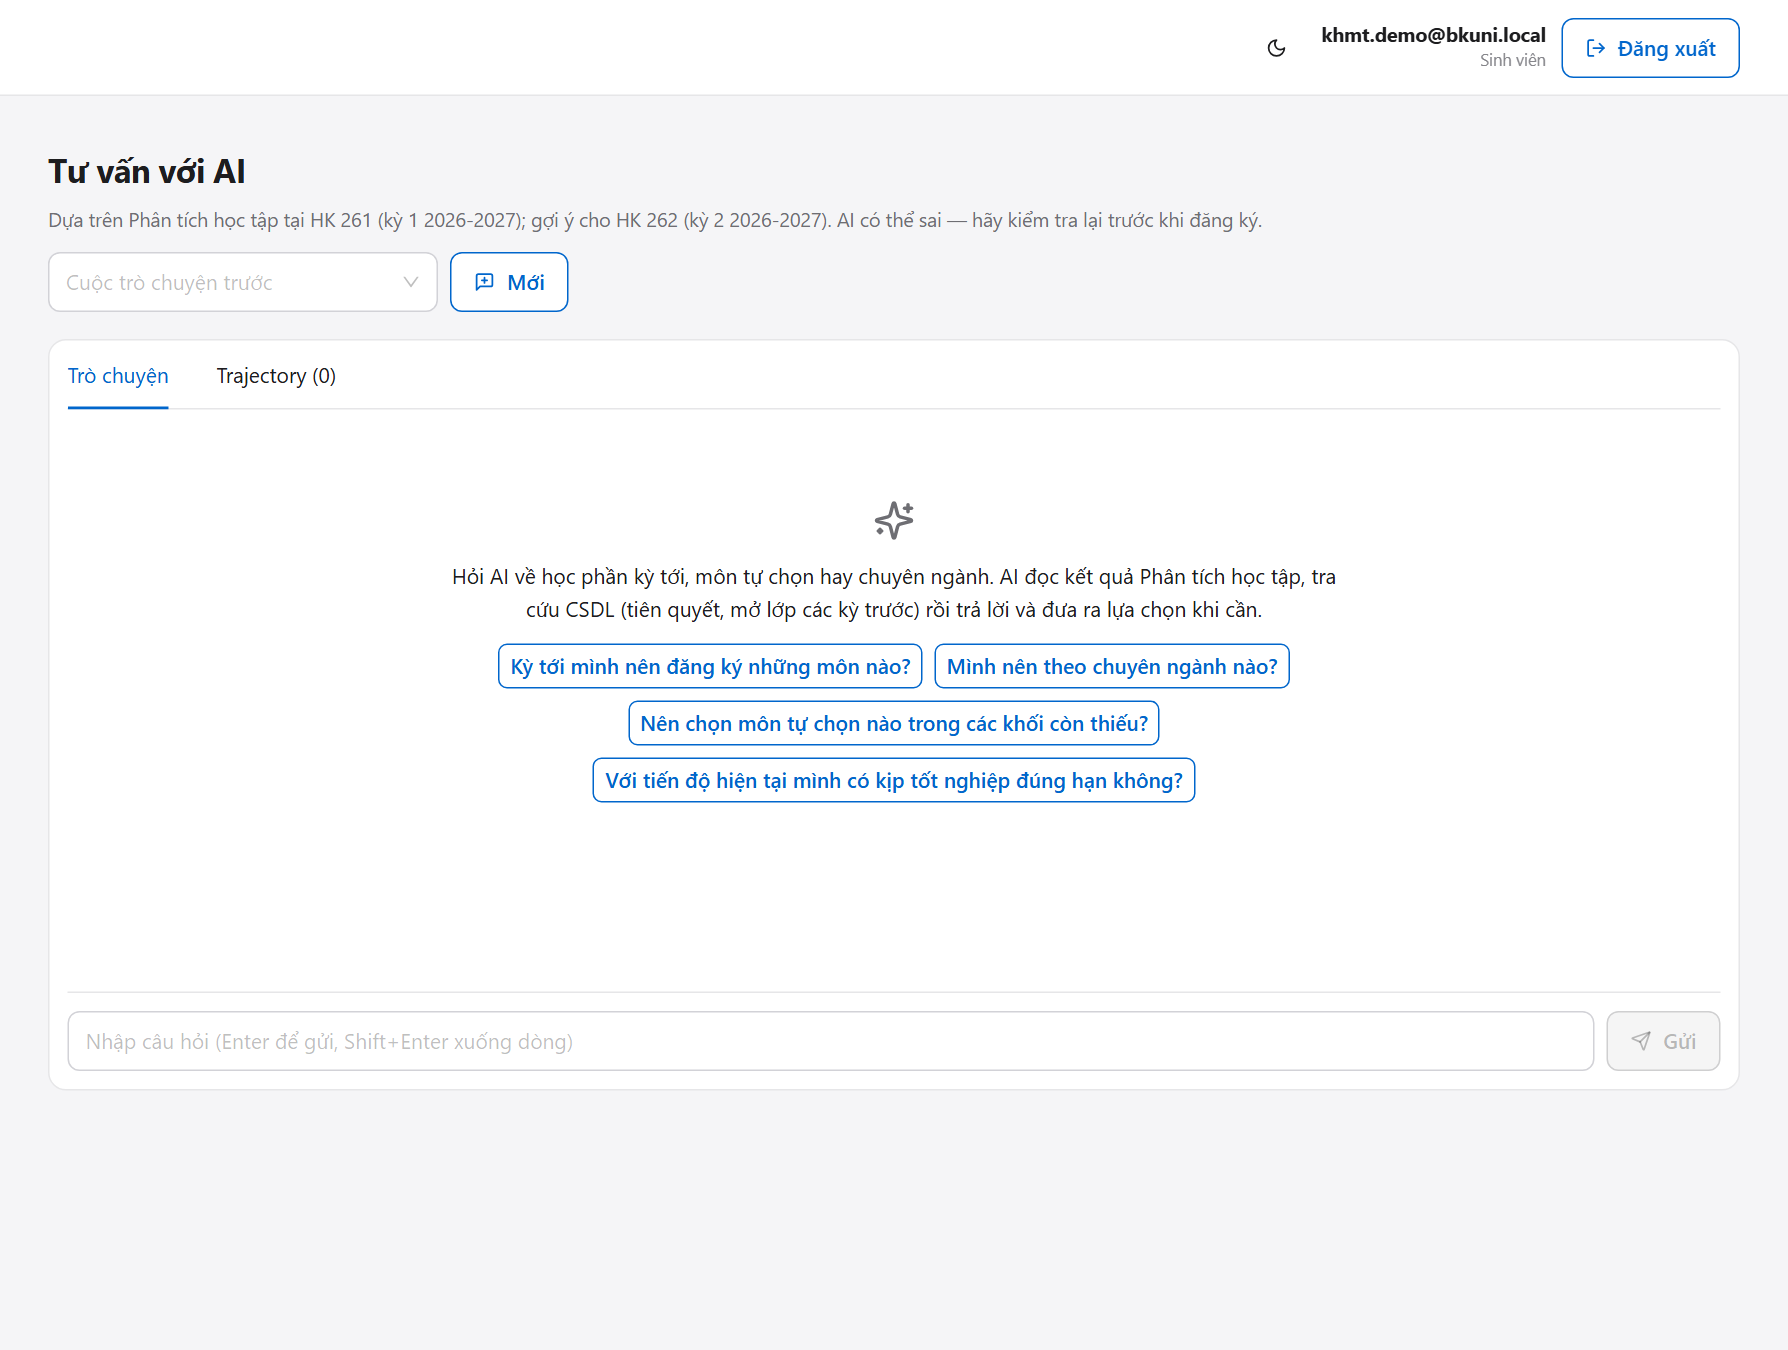
\includegraphics[width=\textwidth]{image/ui/advisor-empty.png}
    \caption{The AI Advisor page when starting a new conversation}
    \label{fig:ui-advisor-empty}
\end{figure}

After a question is sent, the advisor reads the analysis, queries the database through its tools and replies in the chat thread, as illustrated in Figure~\ref{fig:ui-advisor-chat}. The student's question appears on the right and the answer on the left. Besides the written explanation, the answer contains a list of suggested courses, each displayed as a card with its priority, the reason for the suggestion, a summary of its outline (exam format and estimated study hours), and tags indicating whether the student meets its requirements and how likely it is to be offered next semester.

\begin{figure}[H]
    \centering
    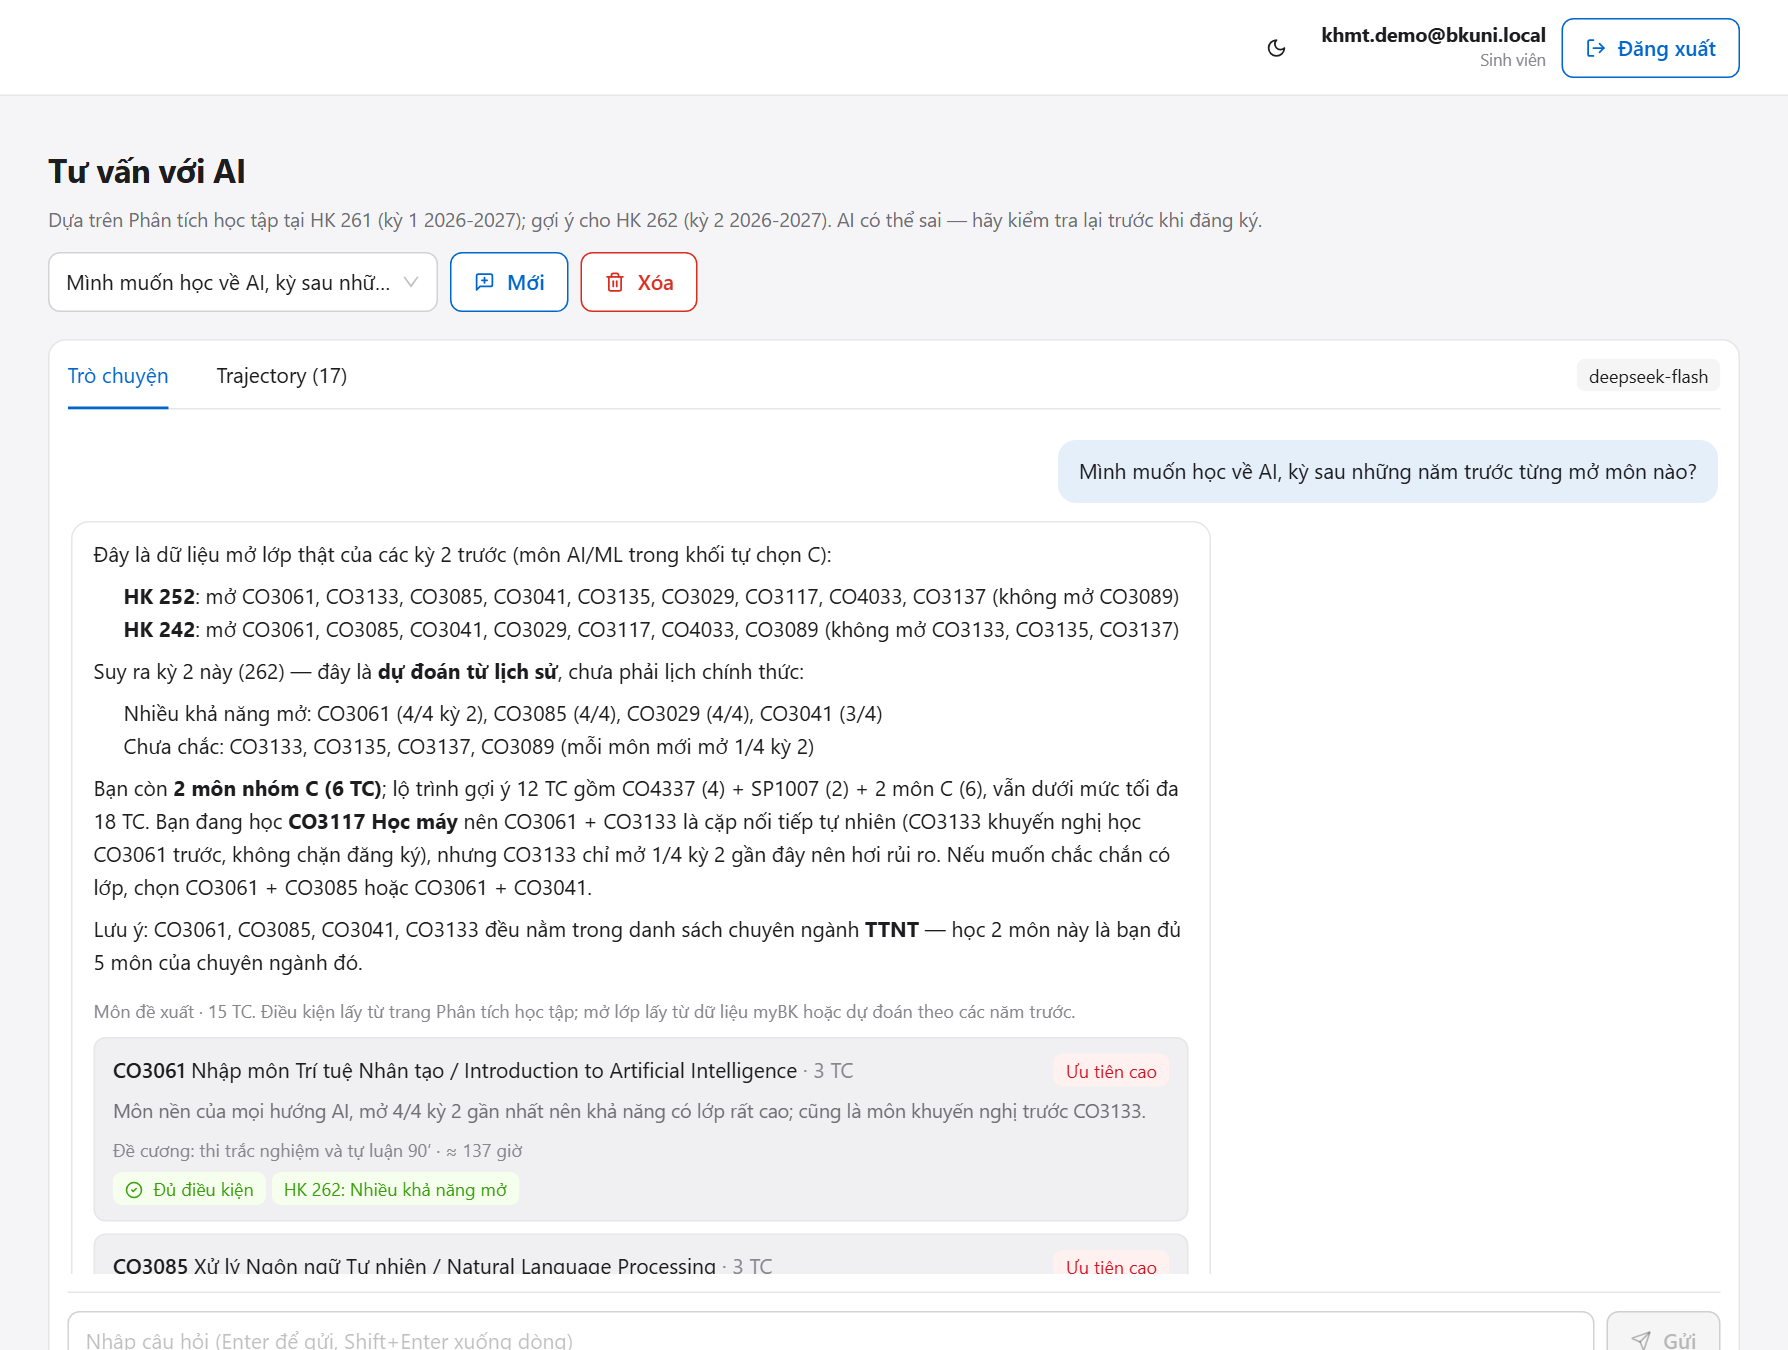
\includegraphics[width=\textwidth]{image/ui/advisor-chat-top.png}
    \caption{An answer of the AI advisor with suggested courses}
    \label{fig:ui-advisor-chat}
\end{figure}

When the advisor needs more information to give a better answer, it asks the student clarifying questions with predefined options instead of guessing, as shown in Figure~\ref{fig:ui-advisor-choices}. Each option comes with a short explanation, and an additional text box lets the student give a different answer before clicking \emph{Gửi lựa chọn} (Send choices). Follow-up questions are also suggested at the end of the answer so that the conversation can continue naturally.

\begin{figure}[H]
    \centering
    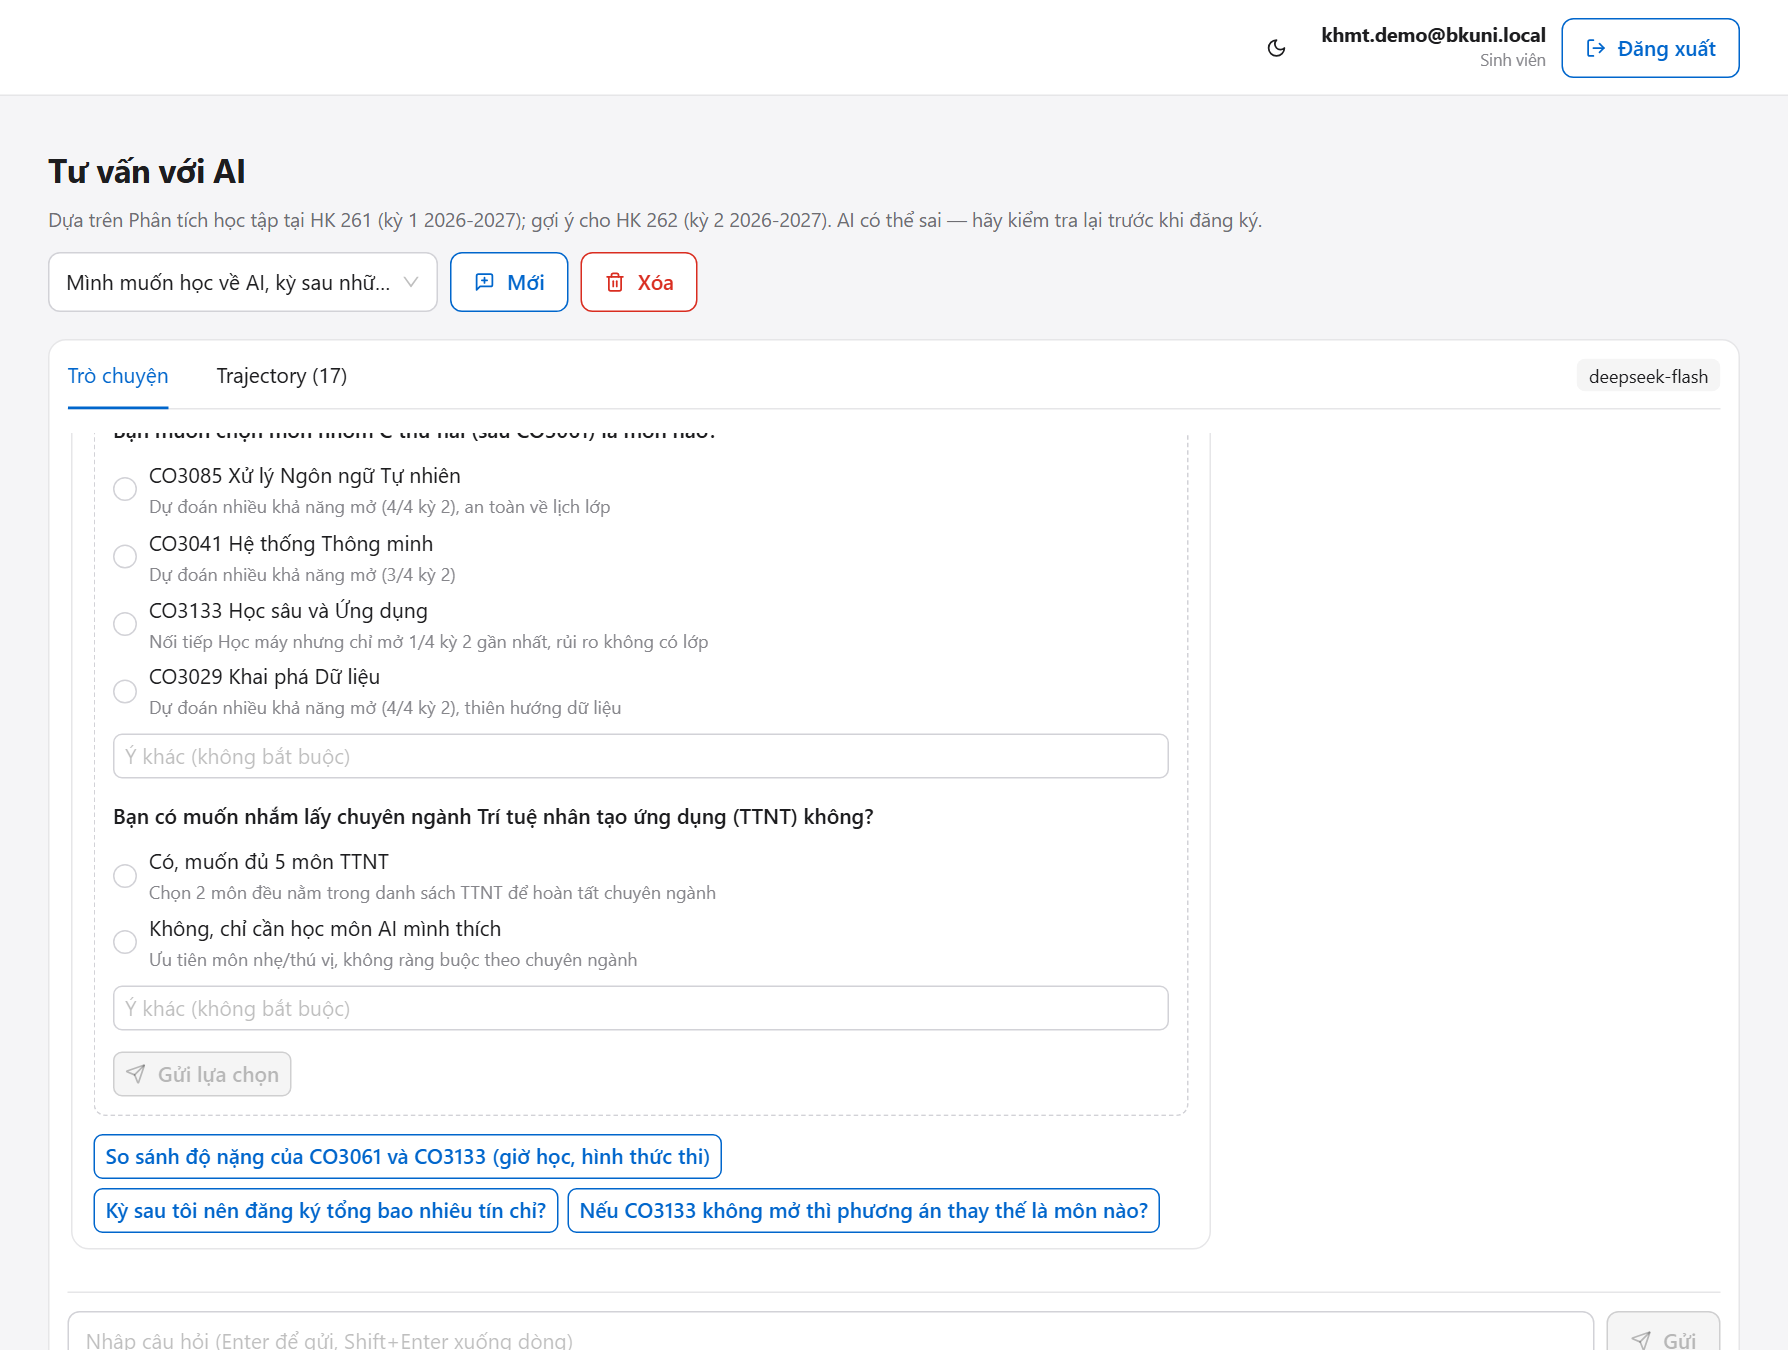
\includegraphics[width=\textwidth]{image/ui/advisor-chat-bottom.png}
    \caption{Clarifying questions and follow-up suggestions in the Chat tab}
    \label{fig:ui-advisor-choices}
\end{figure}

To make the advisor transparent and easy to verify, the Trajectory tab, shown in Figure~\ref{fig:ui-advisor-trace}, records every step the agent performed to produce its answers. The steps are grouped by turn and labelled by their role: the system prompt, the analysis context, the user's message, the model's reasoning together with the tools it decided to call, each tool call with its arguments and result, and the final answer. Each row can be expanded to show its full content, and the token usage, cache hits and duration of each step are displayed on the right. A summary at the top shows the number of turns, requests, tool calls, total tokens and the cache-hit rate, and the steps can be filtered to show only model or tool steps.

\begin{figure}[H]
    \centering
    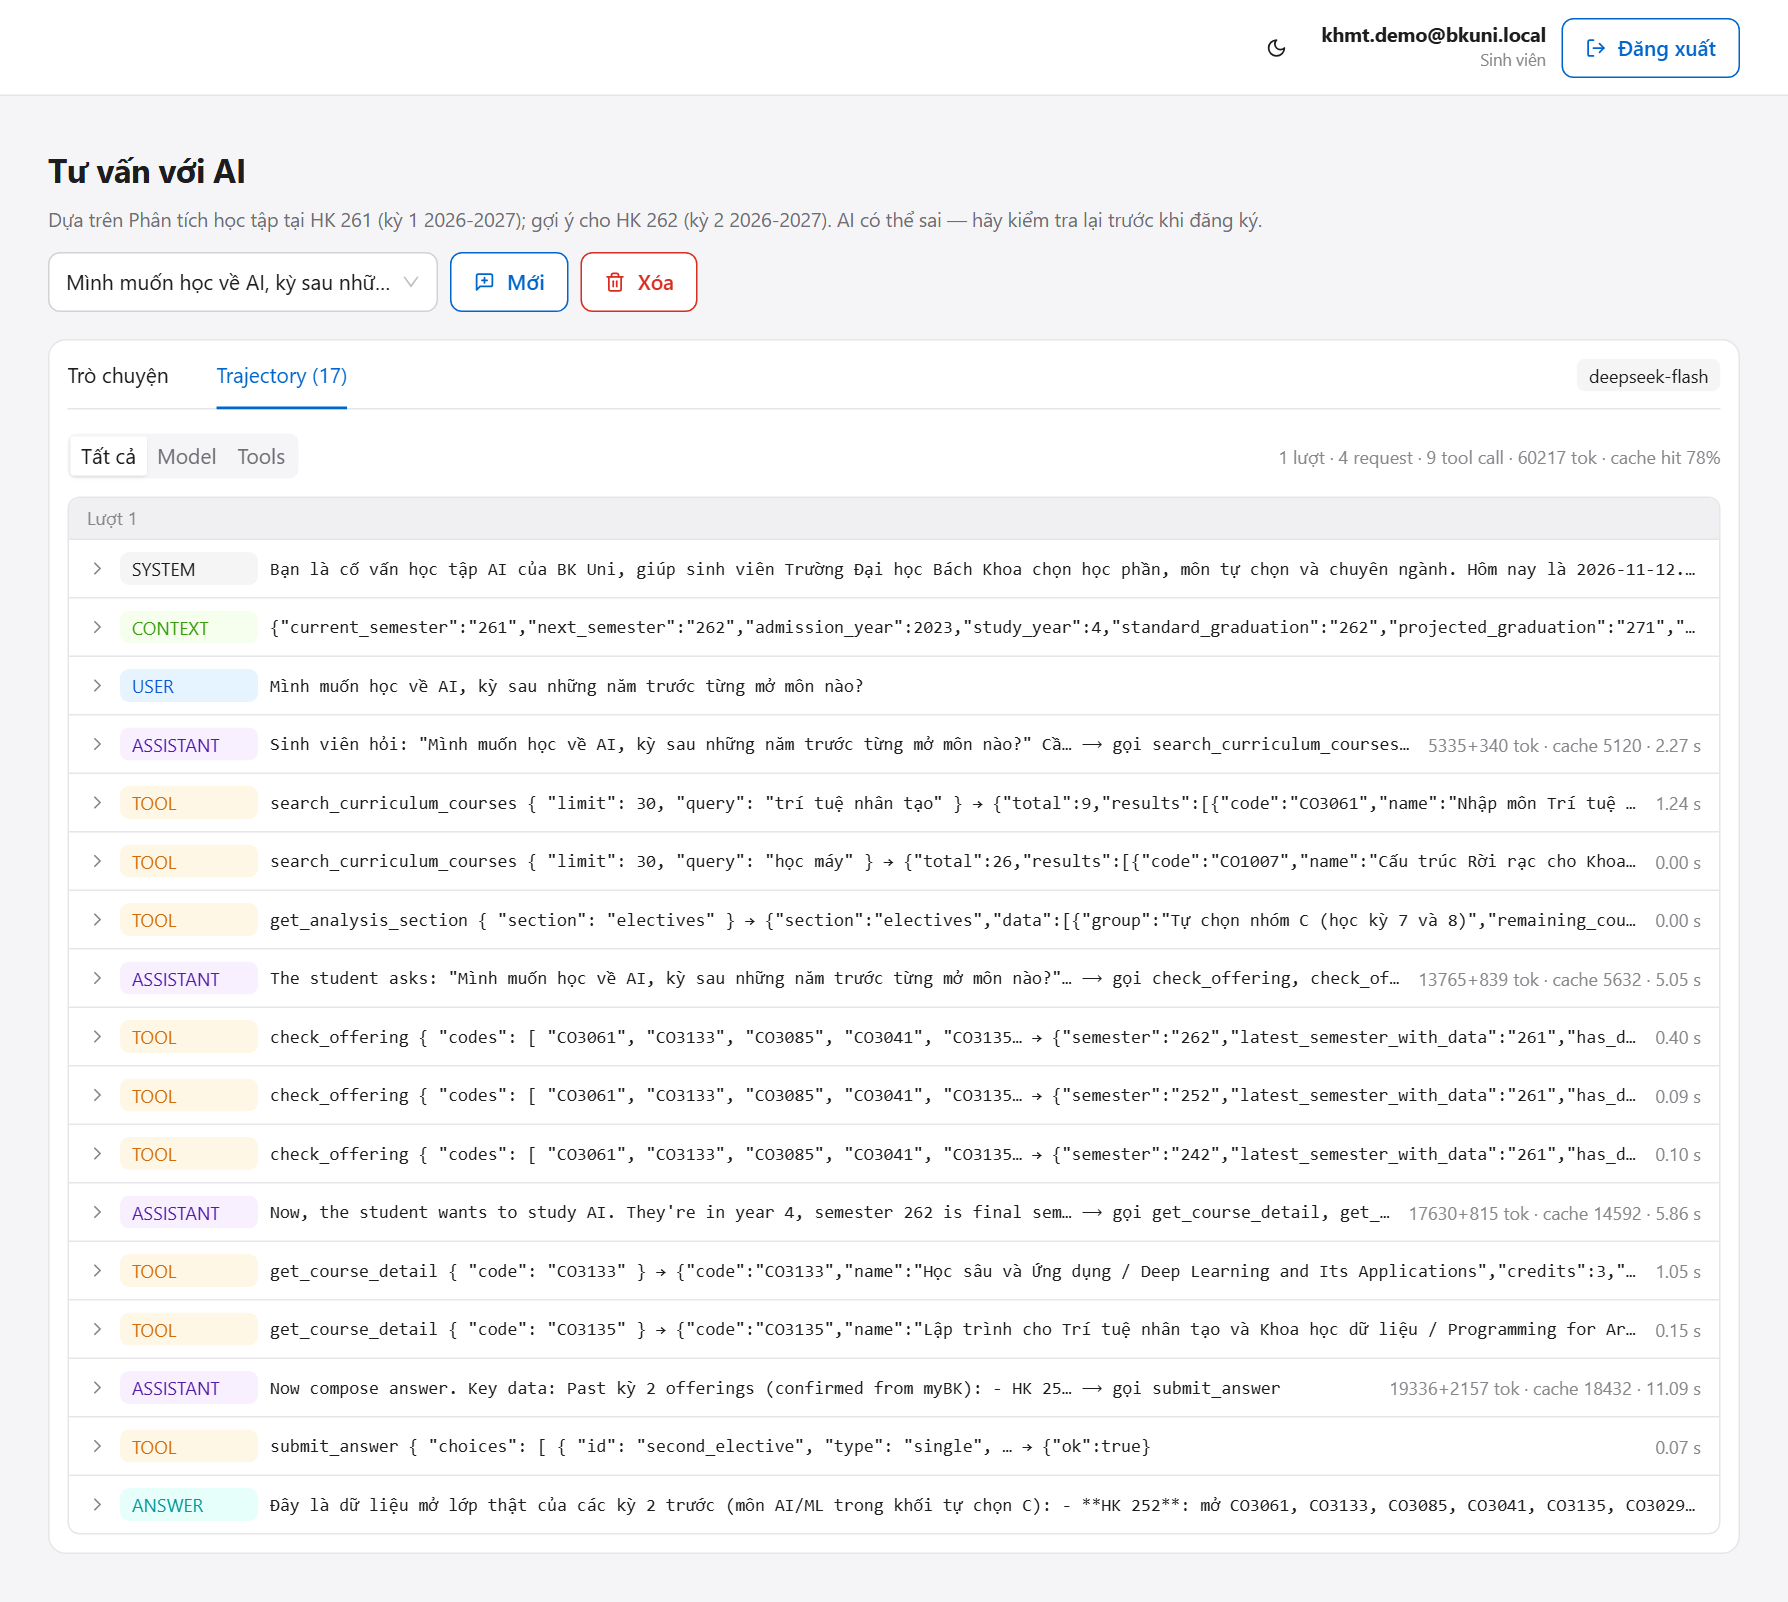
\includegraphics[width=\textwidth]{image/ui/advisor-trace.png}
    \caption{The Trajectory tab of the AI Advisor}
    \label{fig:ui-advisor-trace}
\end{figure}

\subsubsection{Personal Profile Page}
\label{subsubsec:ui-profile}

Lastly, the \emph{Hồ sơ cá nhân} (Personal Profile) page, shown in Figure~\ref{fig:ui-profile}, lets students keep their information up to date. The page consists of three cards. The \emph{Tài khoản đăng nhập} (Sign-in account) card shows the email and role of the account. The \emph{Thông tin sinh viên} (Student information) card is a form containing the full name, student number, phone number, date of birth, admission year, credit target, curriculum and contact address; short hints under the fields explain their constraints, such as the uniqueness of the student number. Among these fields, the curriculum, admission year and credit target are especially important, since they determine the courses shown on the Course List page, the semester used in the Learning Analysis and the number of credits placed in each semester of the suggested roadmap. Finally, the \emph{Chương trình đang theo học} (Current curriculum) card summarizes the selected curriculum, including its code, name, major, faculty, cohort and credit limits per semester, with a shortcut to start planning.

\begin{figure}[H]
    \centering
    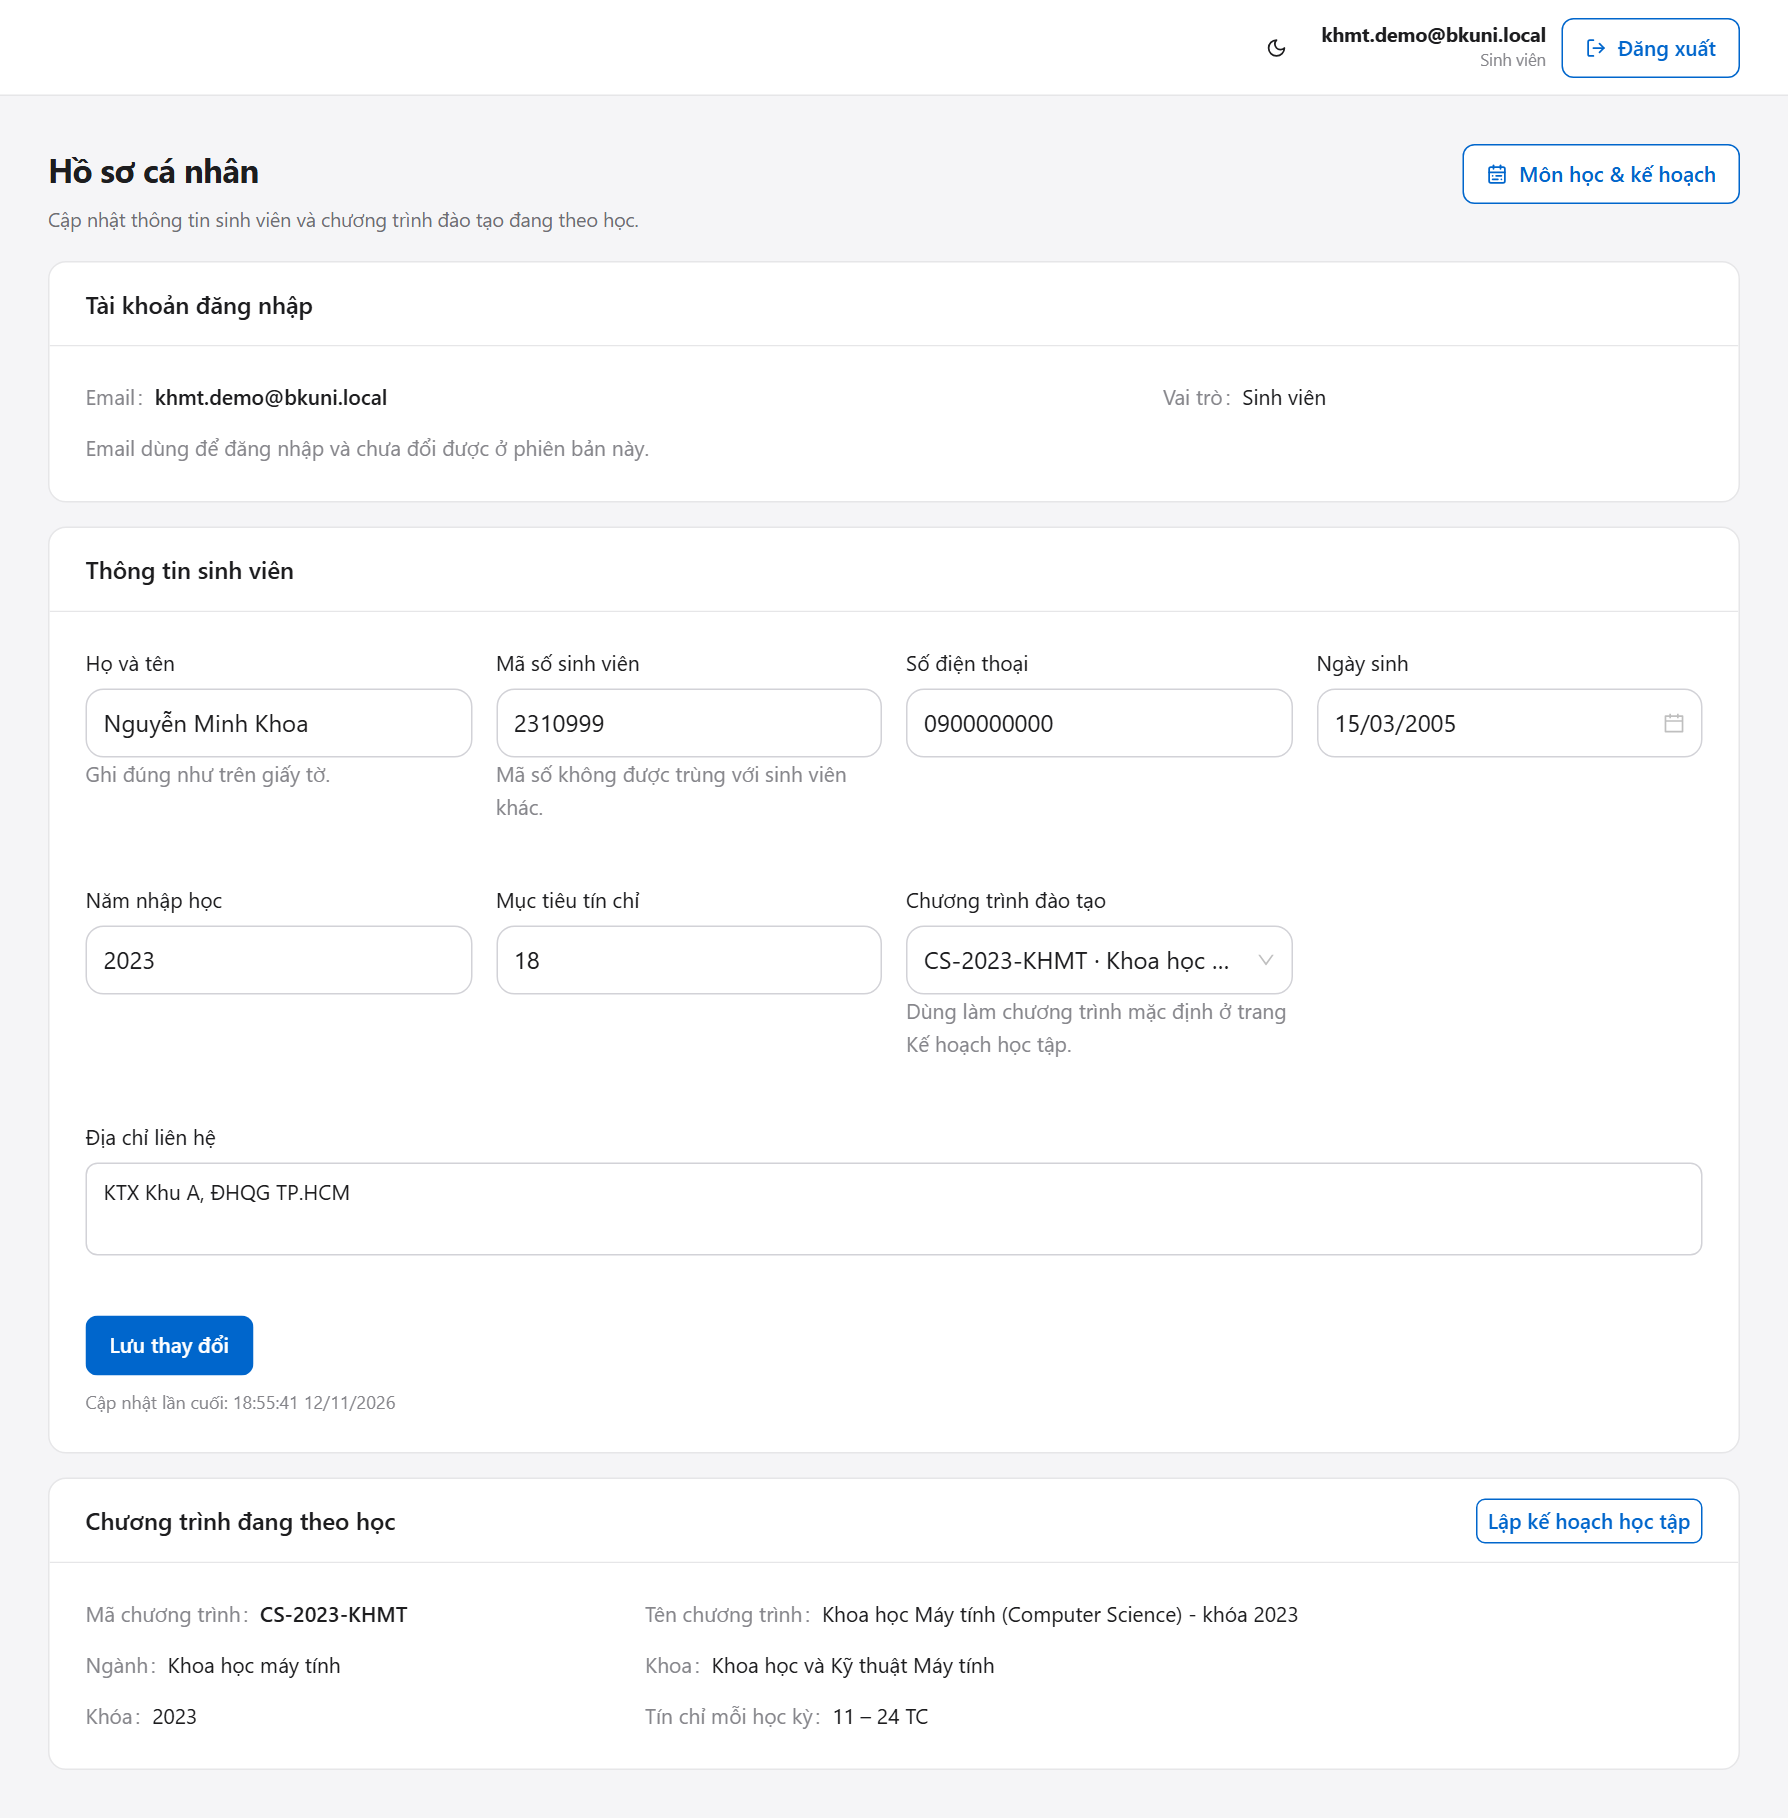
\includegraphics[width=\textwidth]{image/ui/profile.png}
    \caption{The Personal Profile page}
    \label{fig:ui-profile}
\end{figure}

\subsection{AI Advisor: Retrieval-Augmented Generation}
\label{subsec:rag}

This section specifies the algorithm behind the AI Advisor page presented in Section~\ref{subsec:ui-design}. The advisor answers open-ended questions in natural language, such as which elective fits a specialization, whether a course is heavy, or how to balance a semester. A large language model (LLM) plans a \emph{trajectory} of tool calls that retrieve the Student's analysis results and curriculum data, and then writes an answer that the backend validates before showing it. The advisor follows a strict division of labour with the rule-based code of the system (Section~\ref{subsubsec:architecture-overview}): the progress analysis computed from curriculum rules is the source of truth for eligibility, outstanding requirements and bottleneck courses, while the LLM explains, prioritizes and asks follow-up questions. The advisor never decides on its own whether a Student may take a course; it reads that decision from the analysis results.

\subsubsection{Motivation and Design Principles}

An LLM on its own is unsuitable for academic advising. It does not know a specific curriculum, it may invent course codes, credit values or prerequisite relations, and its answers cannot be checked. Retrieval-Augmented Generation (RAG) addresses this by retrieving relevant information from a trusted source and placing it in the model's context before the answer is generated.

Classic RAG retrieves text passages from a vector index by embedding similarity. BK Uni uses an \emph{agentic, tool-based} variant instead, because its knowledge is mostly structured and relational (courses, rules, groups, statuses, offering history) and must be exact rather than merely similar. The model is given a set of tools, each backed by a database query or by the analysis results, and decides during the conversation which tools to call and with which arguments. The design follows four principles:
\begin{itemize}
    \item \textbf{Grounding:} every course code, name, credit value or rule mentioned in an answer must come from the context or from a tool result (FR-7.2).
    \item \textbf{Separation of decision and explanation:} eligibility, outstanding requirements and bottleneck courses are computed by rule-based code and given to the model as facts; the model only interprets them.
    \item \textbf{Mixed initiative:} when information is missing or several reasonable options exist, the model asks the Student a structured question instead of choosing on the Student's behalf (FR-7.3).
    \item \textbf{Verifiability:} the final answer is structured data checked by the backend, and the whole trajectory that led to it is stored, so every answer can be audited afterwards.
\end{itemize}

\subsubsection{Retrieval Sources}

The information available to the model in a turn comes from three layers, ordered from the most general to the most specific:
\begin{enumerate}
    \item \textbf{System prompt (domain knowledge).} A fixed instruction that defines the advisor's role and encodes domain knowledge that cannot be inferred from the data: the meaning of prerequisite, prior and corequisite relations; how specializations are obtained (a Student keeps a specialization only while every elective taken from the base group belongs to its list); how physical-education requirements are satisfied by concrete sports courses; and the priority order for recommendations (failed courses to retake, overdue required courses, bottleneck courses that unlock many others, required courses on schedule, then electives), capped by the semester's credit limit.
    \item \textbf{Analysis context (the Student's state).} A compact JSON summary of the Student's learning analysis, attached to the user message inside a \texttt{<context>} block. It contains the current and next semester, credit overview and capacity, warnings, failed and overdue courses, the number of required courses left, elective-group and specialization progress, the list of courses eligible for the next semester, the top bottleneck courses, the next step of the roadmap and unmet graduation regulations. To save tokens, the context is re-sent only when the analysis changes: the backend stores a SHA-256 hash of the full analysis with the conversation and attaches a new context block only when the hash differs.
    \item \textbf{Tools (details on demand).} Everything that does not fit in the summary is retrieved through the tools in Table~\ref{tab:advisor-tools}, which the model may call several times and in parallel within a turn.
\end{enumerate}

\begin{longtable}{|>{\raggedright\arraybackslash}p{0.32\textwidth}|>{\raggedright\arraybackslash}p{0.19\textwidth}|>{\raggedright\arraybackslash}p{0.39\textwidth}|}
\caption{Tools available to the AI advisor}
\label{tab:advisor-tools}\\
\hline
\textbf{Tool} & \textbf{Data source} & \textbf{Purpose} \\
\hline
\endfirsthead
\hline
\textbf{Tool} & \textbf{Data source} & \textbf{Purpose} \\
\hline
\endhead
\texttt{get\_analysis\_section} & Analysis results & Returns one section of the analysis in full (for example \texttt{eligible\_next}, \texttt{blocked\_next} with missing courses, \texttt{electives}, \texttt{roadmap}); the primary source for eligibility and progress. \\
\hline
\texttt{get\_course\_detail} & Database & Course information, recommended semester, prerequisite, prior and corequisite relations with the Student's status for each related course, courses it unlocks, containing elective groups and specializations, and offering history. \\
\hline
\texttt{check\_offering} & Offering history (myBK) & Whether up to 30 courses are offered in a given semester; confirmed when the semester's data exists, predicted otherwise. \\
\hline
\texttt{get\_course\_outline} & Course outlines (myBK) & Condensed course outline: objectives, weekly content, learning outcomes, grading scheme, exam format, study hours, materials, and outline conditions placed next to curriculum conditions. \\
\hline
\texttt{search\_curriculum\_\allowbreak courses} & Database and outlines & Searches the Student's curriculum by code, name keyword or topic in the outline content (accent-insensitive), returning statuses, groups and specializations. \\
\hline
\texttt{get\_specialization\_\allowbreak detail} & Database & Courses of a specialization, grouped by block with the required number of courses or credits, together with the Student's status for each course. \\
\hline
\texttt{search\_\allowbreak outlines} & Search index (or database) & Full-text search over the whole content of the course outlines, by topic, skill or tool, ranked by relevance with highlighted excerpts; can be limited to the Student's curriculum and filtered by laboratory work, projects or final-exam format. \\
\hline
\texttt{find\_similar\_\allowbreak courses} & Search index & Courses whose outlines are closest in content to a given course, with the characteristic keywords of that course; used for alternatives within an elective group or for what to study next. \\
\hline
\texttt{get\_senior\_free\_\allowbreak elective\_tips} & Curated list and database & Free-elective courses recommended by students of earlier cohorts (unofficial experience), with their credits, next-semester offering, the Student's status, and the free-elective requirement of the curriculum. \\
\hline
\texttt{submit\_answer} & -- & Submits the final structured answer; must be called exactly once to end the turn. \\
\hline
\end{longtable}

All tools are read-only and run inside the backend under the identity of the current Student. Their arguments only select what to read, never whose data, because the Student and the curriculum are fixed by the authenticated session rather than chosen by the model. Each tool result is serialized as JSON and truncated to 16{,}000 characters before being returned to the model.

When the offering data of the target semester is not yet available, \texttt{check\_offering} predicts it from the four most recent semesters of the same type (first semester, second semester or summer) for which data exists. Let $h$ be the number of those semesters in which the course was opened. The verdict is \emph{likely} if $h \ge 3$, \emph{uncertain} if $1 \le h \le 2$, \emph{unlikely} if $h = 0$ but the course has been opened in a semester of that type before, and \emph{never} if it has not. The advisor is instructed to present these verdicts as predictions from history, not as an official timetable.

\subsubsection{Agent Trajectory}

A conversation is a sequence of \emph{turns}, and each turn produces a \emph{trajectory}: an ordered list of steps
\[
  \tau = \langle s_1, s_2, \dots, s_n \rangle,
\]
where each step $s_i$ has one of the roles \texttt{system}, \texttt{context}, \texttt{user}, \texttt{assistant}, \texttt{tool}, \texttt{answer} or \texttt{error}. An \texttt{assistant} step holds the model's output for one call: its visible content, its reasoning trace and the tool calls it requested, together with token usage and latency. A \texttt{tool} step holds the name, arguments, result and execution time of one tool call. The turn ends with exactly one \texttt{answer} step, or with an \texttt{error} step if it could not be completed. Algorithm~\ref{alg:advisor-turn} describes how a turn is executed.

\begin{algorithm}[H]
\caption{One turn of the AI advisor}
\label{alg:advisor-turn}
\KwIn{Student $u$, conversation $c$ with stored steps $\tau_{\mathit{prev}}$, question $q$, analysis $A$}
\KwOut{Validated answer $a$, appended to $c$ as new steps}
$M \leftarrow \textsc{Replay}(\tau_{\mathit{prev}})$\tcp*{rebuild message history}
\If{$c$ has no system step}{record and prepend the system prompt to $M$}
\If{$\mathrm{SHA256}(A) \neq c.\mathit{hash}$}{
  $x \leftarrow \textsc{Summarize}(A)$; record a \texttt{context} step; $c.\mathit{hash} \leftarrow \mathrm{SHA256}(A)$\;
}
append $q$ (wrapped with $x$ if present) to $M$ and record a \texttt{user} step\;
$\mathit{rejected} \leftarrow \mathit{false}$\;
\For{$r \leftarrow 1$ \KwTo $R_{\max}=8$}{
  $\mathit{res} \leftarrow \textsc{LLM}(M, \mathit{tools})$; record an \texttt{assistant} step; append $\mathit{res}$ to $M$\;
  \If{$\mathit{res}$ requests no tool call}{
    $d \leftarrow \mathit{res}.\mathit{content}$\tcp*{plain-text draft}
    \textbf{break}\;
  }
  \ForEach{tool call $(f, \mathit{args}) \in \mathit{res}$}{
    \eIf{$f = \texttt{submit\_answer}$}{
      $(a, E) \leftarrow \textsc{Validate}(\mathit{args}, \mathit{lenient}=\mathit{rejected})$\;
      \lIf{$a$ is accepted}{$\mathit{out} \leftarrow \{\mathit{ok}\}$}
      \lElse{$\mathit{out} \leftarrow E$; $\mathit{rejected} \leftarrow \mathit{true}$}
    }{
      $\mathit{out} \leftarrow \textsc{Execute}(f, \mathit{args}, u)$\;
    }
    record a \texttt{tool} step; append $\textsc{Truncate}(\mathit{out})$ to $M$\;
  }
  \lIf{an answer $a$ was accepted}{record an \texttt{answer} step and \Return{$a$}}
}
$a \leftarrow \textsc{FormatJson}(d, q, \text{tool results of this turn})$\tcp*{fallback}
record an \texttt{answer} step and \Return{$a$}\;
\end{algorithm}

Within one round the model may request several tool calls at once, for example \texttt{check\_offering} for all candidate courses together with \texttt{get\_course\_outline} for the ones whose workload matters. A typical trajectory therefore has two or three rounds: the model reads the context, retrieves the details it needs, and submits its answer. The bound $R_{\max} = 8$ prevents a model that keeps calling tools from running indefinitely. Any exception raised while the turn is being executed, including an unreachable or timed-out AI service, is recorded as an \texttt{error} step, and no answer is fabricated (FR-7.6).

\subsubsection{Answer Validation and Enrichment}

The final answer is not free text but a JSON object passed as the argument of \texttt{submit\_answer}, with four fields:
\begin{itemize}
    \item \texttt{message}: a short answer in Vietnamese, with light formatting;
    \item \texttt{recommendations}: a list of courses, each with a code, a one- or two-sentence reason and a priority (\emph{high}, \emph{medium} or \emph{low});
    \item \texttt{choices}: structured follow-up questions of type \emph{single}, \emph{multiple} or \emph{text}, each option with a short description of its consequences;
    \item \texttt{suggestions}: up to three useful follow-up questions.
\end{itemize}

The backend first normalizes this object against the schema and then \emph{enriches} each recommendation with facts computed by code rather than by the model: the course name and credits from the database, whether the course belongs to the curriculum, its eligibility and missing conditions from the analysis results, its offering verdict for the next semester, and a short summary of its course outline. The interface displays these verified facts next to the model's reason, so a wrong statement in the reason is easy to spot.

Validation includes a self-correction step. If the answer refers to a course code that does not exist or violates the schema, the first submission is rejected and the list of errors is returned to the model as the tool result, so it can correct itself in the next round. If a later submission still contains errors, it is accepted \emph{leniently}: the invalid parts are dropped and a note stating what was removed is attached, so that a single wrong code does not discard an otherwise useful answer.

If the model ends a round with plain text instead of calling \texttt{submit\_answer}, or reaches the round limit, a fallback formatter is used. The backend makes a separate call in JSON mode, with reasoning disabled, that receives the Student's question, the draft answer and the tool results collected during the turn as evidence, and asks for the same schema. The result goes through the same validation. If two attempts fail, the draft text is returned with a note saying it could not be structured. Each answer records whether it came from \texttt{submit\_answer} or from the fallback formatter.

\subsubsection{Trajectory Persistence and Replay}

Every step is stored as soon as it is produced in the \texttt{advisor\_steps} table, ordered by a per-conversation sequence number that is unique within the conversation. This serves three purposes. First, it is the conversation memory: at the start of each turn the message history is rebuilt from the stored steps rather than kept in server memory, so a conversation can be continued at any time, even after the server restarts (FR-7.5). Second, it makes answers auditable: for any answer, it is possible to see exactly which data the model saw, which tools it called with which arguments, what they returned, and how long each step took (NFR-7). Third, the recorded token counts, including tokens served from the provider's prompt cache, make the cost and latency of the advisor measurable.

Replay applies a few rules so that the rebuilt history is always valid for the provider's API:
\begin{itemize}
    \item the model's reasoning trace is kept with each assistant message, as the provider requires when reasoning and tool calling are used together;
    \item calls to the fallback formatter are not part of the main dialogue and are skipped;
    \item a tool call that never received a result, for example because the previous turn failed, is closed with a synthetic ``interrupted'' result;
    \item two consecutive user messages, which occur when a previous turn failed before the model replied, are merged into one;
    \item a context block is replayed together with the user message it was attached to.
\end{itemize}
Finally, only one turn may run on a conversation at a time; a second request on the same conversation is rejected until the first finishes, so the step sequence never interleaves. This lock is kept in the memory of the Backend process, which is sufficient for the current single-instance deployment; running several Backend instances would require moving it to the database or a shared cache.

\subsubsection{Mixed-Initiative Interaction}

When the model returns \texttt{choices}, the interface renders them as selectable options. The Student's selections are sent back with the next message and formatted as a ``choice answers'' block that lists each question with the chosen values or free text. The model then continues advising based on these choices. This lets the advisor fill in information it cannot infer on its own, such as a target specialization, the number of credits the Student is willing to take, or whether summer study is an option. It also keeps decisions with real consequences, such as giving up a specialization by taking an elective outside its list, in the Student's hands.

